\documentclass[a4paper,12pt]{book}
\usepackage[utf8]{inputenc}

\usepackage{lipsum}
%\usepackage[utf8]{inputenc}
%\usepackage{graphicx}
\usepackage{amsmath}
\usepackage{amssymb}
\usepackage{physics}
\usepackage{tcolorbox}
\usepackage{color}   %May be necessary if you want to color links
\usepackage{hyperref}
\usepackage{mathtools}
\usepackage{graphicx} % Allows including images
\usepackage{booktabs} % Allows the use of \toprule, \midrule and \bottomrule in tables
\usepackage{xmpmulti}
\usepackage{calligra}

\begin{document}

\author{Rishi Kumar, Pugazharasu A D}
\title{Notes on Quantum Mechanics}
\date{January 2013}

\frontmatter
\maketitle
\tableofcontents

\mainmatter
% !TeX spellcheck = <none>
\chapter{Mathematical Preliminaries}
This chapter is a discussion of all the mathematical tools and tricks one would require to master Quantum mechanics. Knowledge of basic matrix manipulation and vector calculus is assumed.
\section{Complex Numbers}
A complex number is an order pair ${} \in \mathbb{C}$ where $a,b \in \mathbb{R}$ where we can denote it as $z = a + ib$ where $i = \sqrt{-1}$
\subsection{Addition}
$z_{1} = a_{1} + ib_{1}, \ z_{2} = a_{2} + ib_{2}$
$$z_{1} + z_{2} =  (a_{1} + a_{2}) + i(b_{1} + b_{2})$$
\subsection{Multiplication}
$z_{1} = a_{1} + ib_{1}, \ z_{2} = a_{2} + ib_{2}$
$$z_{1}z_{2} =  (a_{1} + ib_{1})(a_{2} + ib_{2}) = (a_{1}a_{2} - b_{1}b_{2}) + i(a_{1}b_{2} + a_{2}b_{1})$$
\subsection{Properties}
Where, $\mathcal{W}, \mathcal{Z}, \lambda \in \mathbb{C}$
\subsubsection{Commutativity}
$$\mathcal{W} + \mathcal{Z} = \mathcal{Z} + \mathcal{W}$$
$$\mathcal{W}\mathcal{Z} = \mathcal{Z}\mathcal{W}$$
\subsubsection{Associativity}
$$(\mathcal{Z}_1 + \mathcal{Z}_2) + \mathcal{Z}_3 = \mathcal{Z}_1 + (\mathcal{Z}_2 + \mathcal{Z}_3)$$
$$(\mathcal{Z}_1\mathcal{Z}_2)\mathcal{Z}_3 = \mathcal{Z}_1(\mathcal{Z}_2\mathcal{Z}_3)$$
\subsubsection{Identities}
$$\mathcal{Z} + 0 = \mathcal{Z}$$
$$\mathcal{Z}1 = \mathcal{Z}$$
\subsubsection{Additive Inverse}
$$\forall \ \mathcal{Z} \ \exists \ \mathcal{Z}^{-1} \ | \ \mathcal{Z} + \mathcal{Z}^{-1} = 0$$
\subsubsection{Multiplicative Inverse}
$$\forall \  \mathcal{Z} \neq 0 \ \exists \ \mathcal{W} \ | \ \mathcal{Z}\mathcal{W} = 1$$
\subsubsection{Distributive Property}
$$\lambda(\mathcal{W} + \mathcal{Z}) = \lambda\mathcal{W} + \lambda\mathcal{Z}$$
\subsection{Notation}
\textit{\textbf{n-tuple}} refers to an ordered set of $n$ numbers over a field $\mathcal{F}$.\footnote{For our case $\mathcal{F}$ simply refers to $\mathbb{C}$}
\subsection{Wessel Plane}
Complex numbers can be represented on a 2-dimentionsal space similar to $\mathbb{R}^{2}$
\begin{figure}[h]
	\centering
	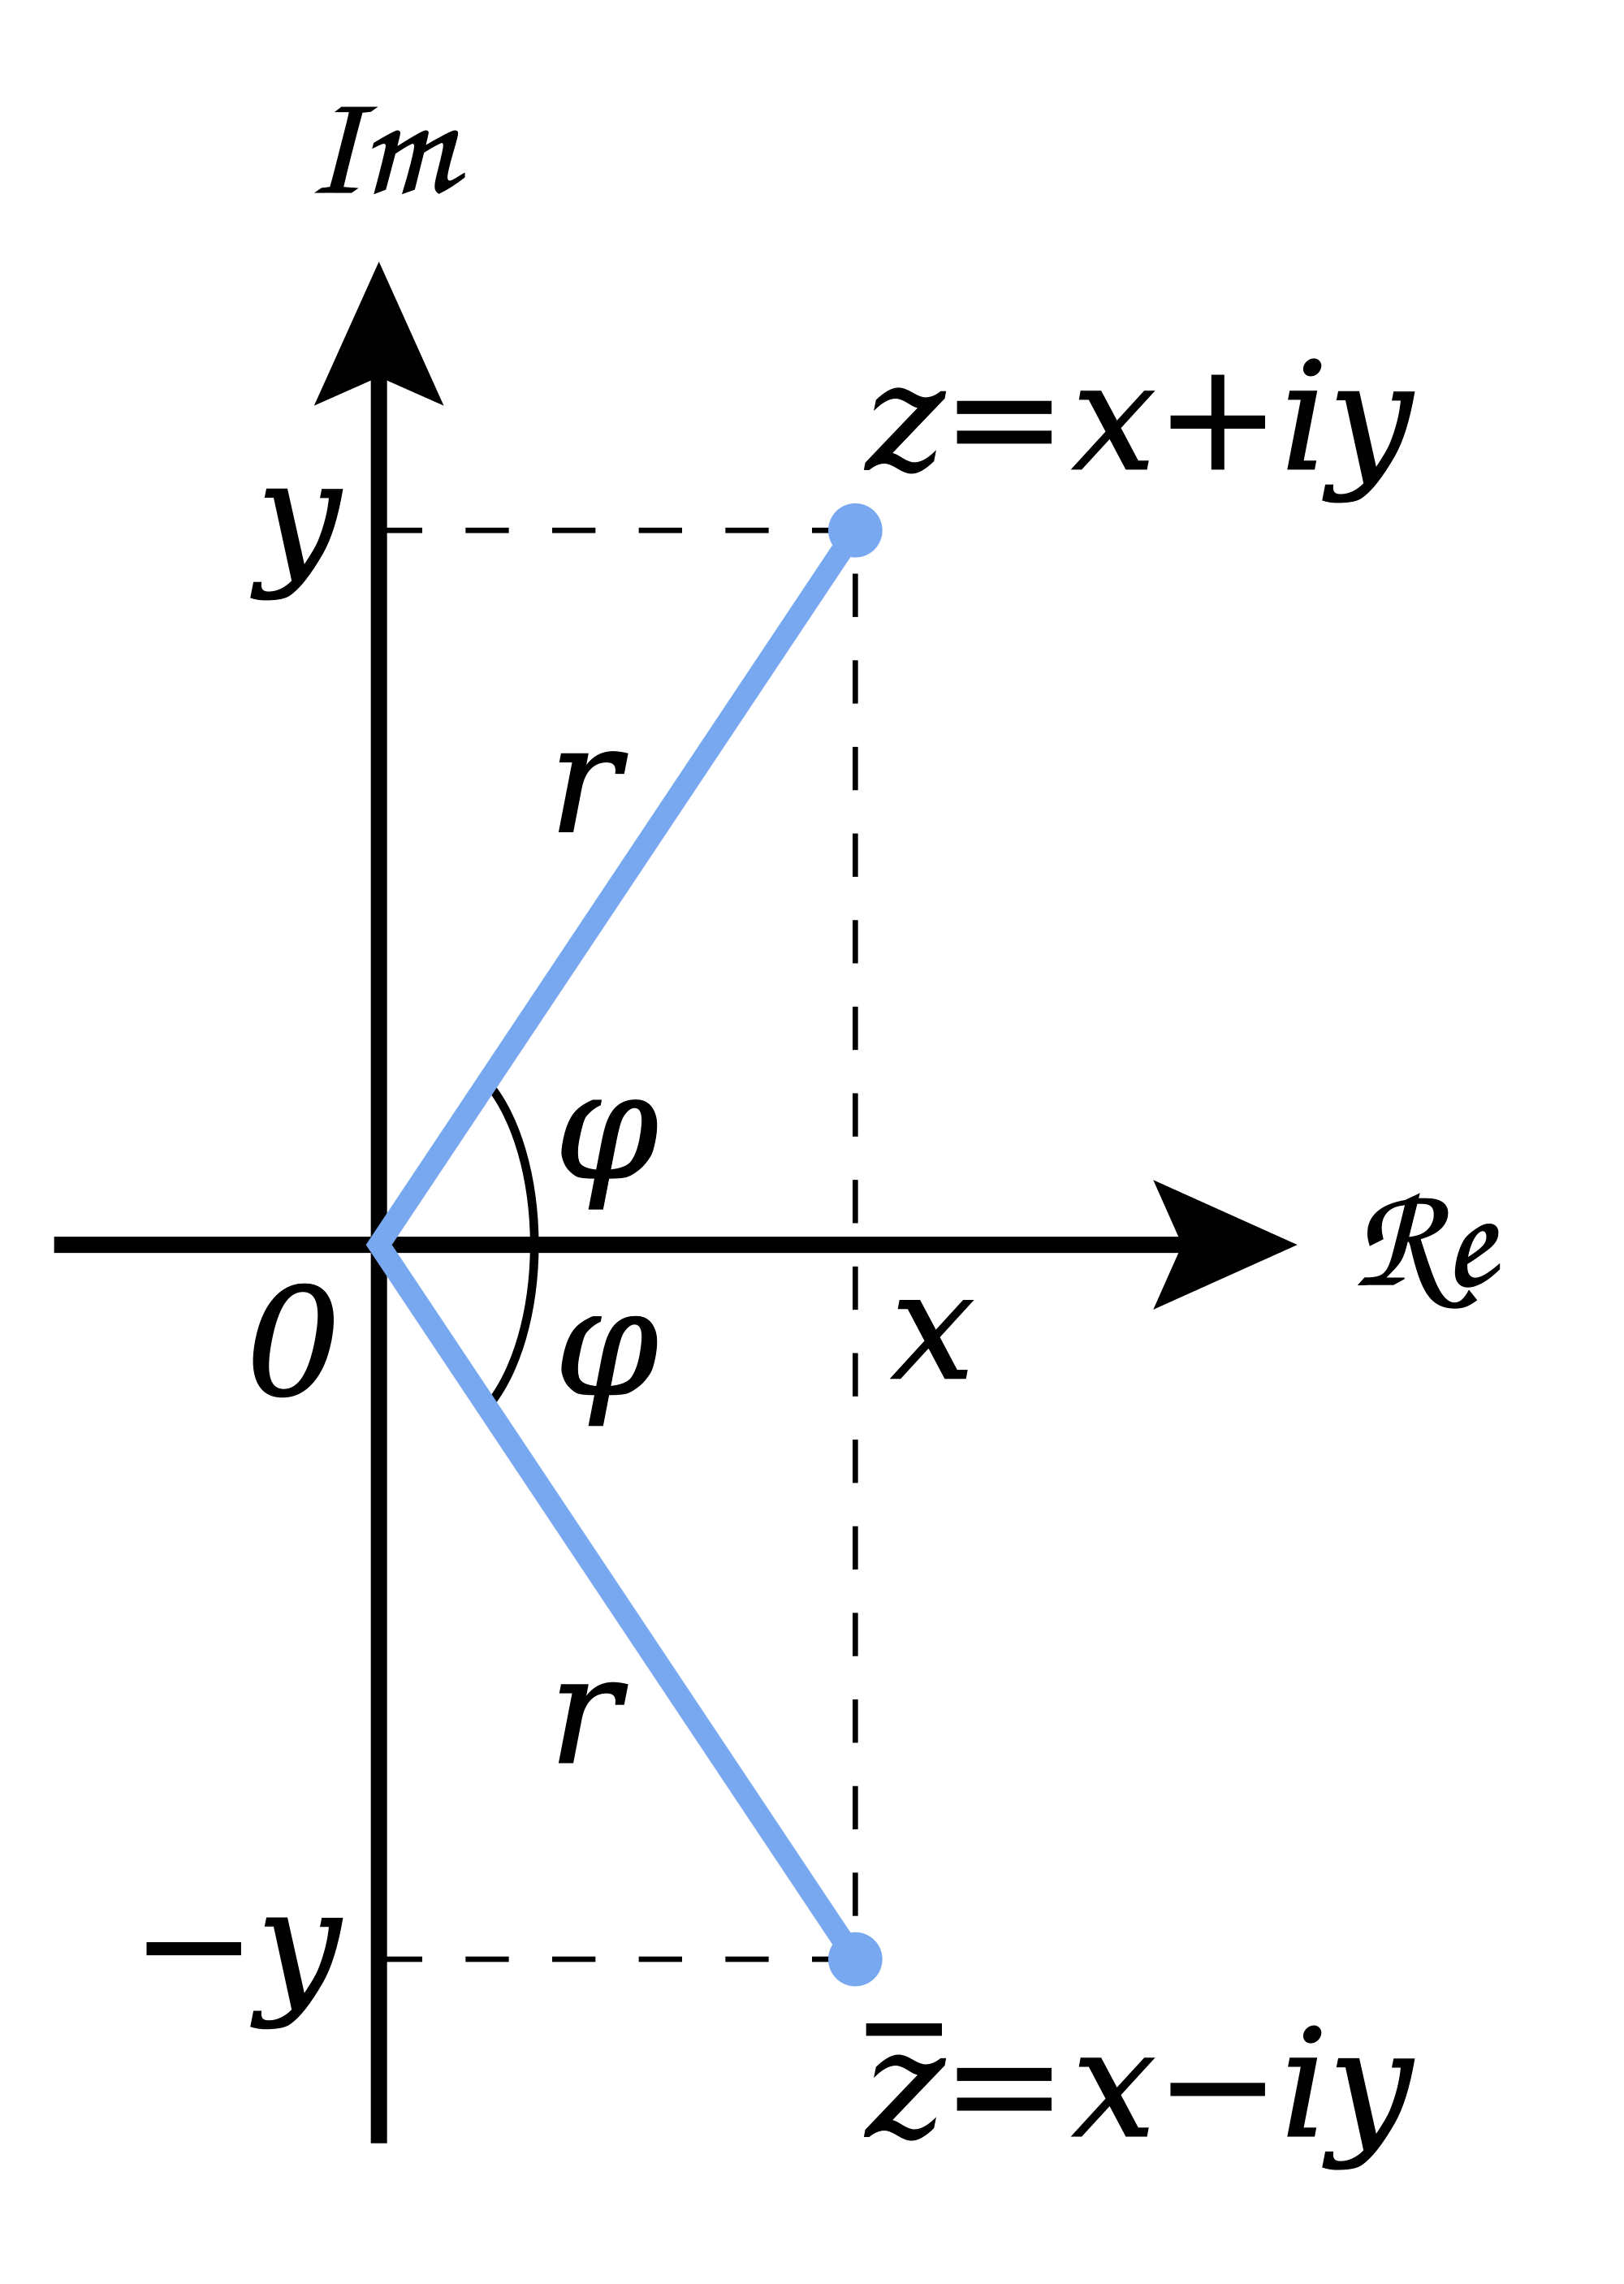
\includegraphics[scale=0.05]{wessel-plane.png}
	\caption{Wessel Plane Plot: (Complex conjugate picture.svg from Wikimedia Commons)}
\end{figure}
\section{Solving PDEs}
What we'll review here is called the variable separable method, 
\section{Linear Vector Spaces} 
A linear vector space or simply a vector space $\mathbb{V}$ is a set along with the regular multiplication and addition operations over a field $\mathcal{F}$, such that the following axioms hold: \footnote{Here, $\alpha , \beta \in \mathcal{F}$ and $\mathcal{U}, \mathcal{V} $ and $\mathcal{W} \in \mathbb{V}$} \\
\subsection{Commutativity}
$$\mathcal{U} + \mathcal{V} = \mathcal{V} + \mathcal{U}$$
\subsection{Associativity}
$$(\mathcal{U} + \mathcal{V}) + \mathcal{W} = \mathcal{V} + (\mathcal{U} + \mathcal{W})$$
$$(\alpha \beta) \mathcal{V} = \alpha (\beta \mathcal{V})$$
\subsection{Additive Identity}
$$\exists \  0 \in \mathbb{V} \ | \ \mathcal{V} + 0 = 0 + \mathcal{V} = \mathcal{V}$$
\subsection{Additive Inverse}
$$\forall \ \mathcal{V} \ \exists \ \mathcal{V}^{-1} \ | \ \mathcal{V} + \mathcal{V} = 0$$
\subsection{Multiplicative identity}
$$\exists \ 1 \in \mathbb{V} \ | \ 1 \mathcal{V} = \mathcal{V}$$
\subsection{Distributive properties}
$$\alpha (\mathcal{U} + \mathcal{V}) = \alpha \mathcal{U} + \alpha \mathcal{V}$$
$$(\alpha + \beta) \mathcal{U} = \alpha \mathcal{U} + \beta \mathcal{U}$$
\section{Inner Product Spaces}
An inner product is simply an operation that takes a Dual $\ket{\psi}$ and it's corresponding vector $\bra{\psi}$ and maps them to $\mathbb{R}$:
$$\braket{expression1}{expression2}$$
\section{Dual Spaces}
\section{Dirac Notation}
Operators are represented with respect to a particular basis (in this case $\{e_{m}, e_{n}\}$) by their matrix elements
\begin{equation}
\langle e_{m}| \hat{O} | {e_n} \rangle = \hat{O}_{mn}
\end{equation}
\section{Subspaces}
Given a vector space $\mathbb{V}$, a subset of its elements that form a vector space among themselves is called a subspace. We will denote a particular subspace $i$ of dimensionality $n_{i}$ by $\mathbb{V}^{n_{i}}_{i}$.\\
   Given two subspaces, and , we define their sum $\mathbb{V}^{n_{i}}_{i} \oplus \mathbb{V}^{m_{i}}_{i} = \mathbb{V}^{l_{i}}_{i}$ \footnote{Here $\oplus$ is the direct sum defined as: } as the set containing:
\begin{enumerate}
\item All the elements of $\mathbb{V}^{n_{i}}_{i}$
\item All the elements of $\mathbb{V}^{m_{j}}_{j}$
\item And all possible linear combinations of the above
\end{enumerate} 
However for the elements of (3), closure is lost. The dimensionality of such a subspace is $n + m$.
\section{Hilbert Spaces}
A Hilbert space $H$ is simply a normed vector space (a Banach space), whose norm is defined as:
\begin{equation} \label{norm}
\norm{V} := \sqrt{\braket{V}{V}}
\end{equation}
This is an axiomatic definition of a Hilbert space, but we are more concerned with the corollaries of it. All the Cauchy sequences \footnote{Defintion} of functions in a Hilbert space always converge to a function that is also a memeber of the space i.e. it is said to be \textbf{complete} which implies that the integral of the absolute square of a function must converege \footnote{we simply state this but a proof can be found in}
\begin{equation}
\int_{a}^{b} \abs{f(x)}^{2} dx < \infty
\end{equation}
Moreover this means that, any function in Hilbert space can eb expressed as a linear combination of other functions i.e. it is closed/complete
\begin{equation}
f(x) = \sum_{n = 1}^{\infty} c_{n} f_{n}(x)
\end{equation}
Where, $c_{n} \in \mathbb{C}$
\section{Linear Operators}
%\section{Eigenvalue Problem}
\section{Eigenfunctions of a Hermitian Operator}

\section{Transformations}
\subsection{Active Tranformation}
In a loose sense this can be thought of as,

\subsection{Passive Tranformation}
From our discussion before it is also clear that the same transformation can be implemented as,
\begin{equation}
\hat{O} \rightarrow U^{\dagger}\hat{O}U
\end{equation}
This is a very different viewpoint, we can understand this by visualizing it to be a 
\subsection{Equivalence of Transformation types}
It's pretty simple to see that both types of transformation constitute the same physical picture. Thus, we can take both viewpoints to mean the same physical transformation in each case, and later on we will see how this leads us two different pictures of Quantum Mechanics and how they are related.
%\section{Functions of Operators}
%\section{Generalization to Infinite Dimensions}
\section{Probability}
\subsection{Discrete Variables}
Suppose we have a frequency distribution 
\begin{equation}
N = \sum_{j=0}^{\infty} N(j)
\end{equation}
The probability of an event $N_{j}$ is defined as,
\begin{equation}
P(j) = \frac{N(j)}{N}
\end{equation}
In probability theory, the sum of all probabilities is 1,
\begin{equation}
\sum_{j = 0}^{\infty}P(j) = \sum_{j = 0}^{\infty}\frac{N(j)}{N} = 1
\end{equation}
The average/mean/expectation value of a value $j$ is given by the formula:
\begin{equation}
	\expval{j} = \frac{\sum j N(j)}{N} = \sum_{j =0 }^{\infty} j P(j)
\end{equation}
and in general, the average of some function of $j$, is given by,
\begin{equation}
\expval{f(j)} = \sum_{j =0 }^{\infty} f(j) P(j)
\end{equation}
The spread of a variable's value from it's mean is called it's variance, written as
\begin{equation}
\sigma^{2} = \expval{{(\Delta j)}^{2}}
\end{equation}
where,
$$\Delta j = j - \expval{j}$$
It's square root is called the standard deviation,
\begin{equation}
\sigma = \sqrt{\expval{{(\Delta j)}^{2}}} =  \sqrt{\expval{j^{2}} - \expval{j}^{2}}
\end{equation}
Which comes from a theorem on variances that we'll find useful later on:
$$\sigma^{2} = \expval{{(\Delta j)}^{2}} = \sum {(\Delta j)}^{2} P(j) = \sum {(j- \expval{j})}^{2} P(j)$$
$$ = \sum (j^{2} - 2j \expval{j} + \expval{j}^{2}) P(j)$$
$$ = \sum j^{2}P(j) - 2 \expval{j} \sum jP(j) + \expval{j}^{2}\sum P(j)$$
$$ = \expval{j^{2}} - 2 \expval{j}\expval{j} + \expval{j}^{2} = \expval{j^{2}} - \expval{j}^{2}$$
\subsection{Continuous Variables}
We now move to a continuous probability distribution, we'll create continuous analogs of all the quantities we just introduced. Let's start with probability, the probability of that $x$ lies between $a$ and $b$
\begin{equation}
	P_{ab} = \int_{a}^{b} \rho(x) dx
\end{equation}
where $\rho(x)$ is the called the probability density i.e. the probability of getting $x$, or more concretely,
$$\rho(x)dx = \text{Probability that an individual is chosend at random lies between } x \text{ and } x + dx$$
Now supposing the rules we held for discrete variables hold, the continuous analogs look like this:
\begin{equation}
	1 = \int_{- \infty}^{\infty} \rho(x) dx
\end{equation}
\begin{equation}
	\expval{x} = \int_{- \infty}^{\infty} x \rho(x) dx
\end{equation}
\begin{equation}
	\expval{f(x)} = \int_{- \infty}^{\infty} f(x) \rho(x) dx
\end{equation}
\begin{equation}
	\sigma^{2} := \expval{(\Delta x)^{2}} = \expval{x^{2}} - {\expval{x}}^{2}
\end{equation}
\section{Expectation Values}
In this section we'll explore how we express the expectation values of a few opeartors. Let's start with the position opeartor in the position representation (i.e. position basis):
\begin{equation} \label{posex}
	\expval{x} = \int_{- \infty}^{\infty} x \abs{\psi(\vec{x}, t)}^{2} dx
\end{equation}
We can differentiate \ref{posex} with respect to time to find the expectation value for "velocity":
$$\frac{d \expval{x}}{dt} = $$
Throwing away 
\begin{equation}
	\expval{v} = \frac{d \expval{x}}{dt} = -\frac{i \hbar}{m} \int \psi^{*} \frac{\partial \psi}{\partial x} dx
\end{equation}
Therefore we can write the expectation value of momentum as,
\begin{equation}
	\expval{p} = m \frac{d \expval{x}}{dt} =  -i \hbar \int \left(\psi^{*} \frac{\partial \psi}{\partial x} \right) dx
\end{equation}
In general, every observable is a function of position and momentum, thus for an observable $\hat{O}(x,p)$, the expectation value is given by,
\begin{equation}
	\expval{\hat{O}(x,p)} = \int \psi^{*} \hat{O}(x,-i \hbar \nabla) \psi dx
\end{equation}
For example, the expectation value of kinetic energy is,
\begin{equation}
\expval{T} = -\frac{\hbar^{2}}{2m} \int \psi^{*} \frac{\partial^{2} \psi}{\partial x^{2}} dx
\end{equation}
Or to sum it up in Dirac notation,
\begin{equation}
	\expval{\hat{O}} = \expval{\hat{O}}{\psi}
\end{equation}
\section{Fourier Analysis}
Fourier analysis is a special case of an integral transform. 
Fourier analysis is the decomposition of a general wave or oscillation into harmonic components.
Because we treat the wave vector as the independent variable of a wave, the Fourier decomposition
is typically done in terms of wave vectors. A Fourier series is a sum of sinusoidal functions, each of
which is a harmonic of some fundamental wave vector or spatial frequency. A Fourier transform is an
integral over a continuous distribution of sinusoidal functions.
A Fourier series is appropriate when the system has boundary conditions that limit the allowed
wave vectors to a discrete set. For a system where the spatial periodicity is 2L, the Fourier decomposition of a general periodic function is the series
\begin{equation}
f(x) = \sum_{-\infty}^{\infty} c_{n}e^{i k_{n}x}
\end{equation}
where,
$$k_{n} = \frac{n \pi}{L}$$
Here $c_{n} \in \mathbb{C}$. All $f(x) \in \mathbb{R}$ can be written as:
\begin{equation}
f(x) = \frac{a_{0}}{2} + \sum^{\infty}_{n=1} \left[a_{n}\cos \left(\frac{n \pi x}{L} \right) + b_{n}\sin \left(\frac{n \pi x}{L}\right) \right]
\end{equation}
Where,
\begin{equation}
	a_{n} = \frac{1}{L} \int_{0}^{2L} f(x) \cos\left(\frac{n \pi x}{L}\right) dx
\end{equation}
\begin{equation}
	b_{n} = \frac{1}{L} \int_{0}^{2L} f(x) \sin\left(\frac{n \pi x}{L}\right) dx
\end{equation}
\begin{equation}
	c_{n} = \frac{1}{2L} \int_{0}^{2L} f(x) e^{-ik_{n}x}dx
\end{equation}
obtained by calculating the overlap integrals (i.e., projections or inner products) of the desired function with the harmonic basis functions. That is provided $f(x)$, obeys the following conditions i.e. \textbf{Dirichlet conditions}:
\begin{itemize}
\item It must be absolutely integrable over a period.
\item It must be of bounded variation in any given bounded interval.
\item It must have a finite number of discontinuities in any given bounded interval, and the discontinuities cannot be infinite.
\end{itemize}
A Fourier transform is appropriate when the system has no boundary conditions that limit the allowed wave vectors. In this case, the Fourier decomposition is an integral over a continuum of wave vectors:
\begin{equation}
	f(x) = \frac{1}{\sqrt{2 \pi}} \int_{-\infty}^{\infty} a(k)e^{ikx}dk
\end{equation}
where  the  expansion  function  $a(k)$  is  complex. To  obtain  the  expansion  function  $a(k)$  for  a  givenspatial function $f(x)$ requires the inverse Fourier transform
\begin{equation}
	a(k) = \frac{1}{\sqrt{2 \pi}} \int_{-\infty}^{\infty} f(x)e^{-ikx}dx
\end{equation}
which is a projection of the spatial function $f(x)$ onto the harmonic basis functions $e^{ikx}/\sqrt{2 \pi}$. The basis functions are orthogonal and normalized in the Dirac sense, which means their projections onto each other are Dirac delta functions
\begin{equation}
\begin{split}
	\frac{1}{2 \pi} & \int_{-\infty}^{\infty} e^{ik^{'}x}e^{-ikx}dx = \delta(k-k^{'})\\
	\frac{1}{2 \pi} & \int_{-\infty}^{\infty} e^{ikx^{'}}e^{-ikx}dk = \delta(x-x^{'})
\end{split}
\end{equation}
\subsection{Parseval’s theorem}
Parseval’s theorem states that the power is the same whether calculated in position space or wave-vector space:
\begin{equation}
\int^{\infty}_{-\infty} \abs{f(x)}^{2}dx = \int^{\infty}_{-\infty} \abs{a(k)}^{2}dk
\end{equation}
\section{Delta Function}
\subsection{The Divergence of $\frac{\hat{r}}{r^{2}}$}
We can see why the divergence is,
\begin{equation}
\nabla . \frac{\hat{r}}{r^{2}} = 0
\end{equation}
But if we calculate this using the Divergence theorem, we find that ,
\begin{equation}
	\oint v .da = \int \left( \frac{\hat{r}}{r^{2}} \right) . \left( r^{2} \sin(\theta) d \theta d \phi \hat{r} \right) = \left( \int_{0}^{\pi} \sin(\theta) d \theta \right) \left( \int_{0}^{2\pi} d \phi \right) = 4 \pi
\end{equation}
This is paradoxical. The issue is that it blows up at $r=0$ but is is neglible everywhere else. How do we fix this? The Dirac Delta functional!
\subsection{The One-Dimensional Dirac Delta Functional}
The Dirac Delta is a functional \footnote{An object that is a map between functions} which we define as,
\begin{equation} \label{deltadef}
\delta(x-a)= 
\begin{cases}
0, & \text{if } x \neq a\\
\infty,              & \text{if } x = a
\end{cases}
\end{equation}
\begin{equation}
\int_{- \infty}^{+ \infty} \delta(x-a) dx = 1
\label{del2}
\end{equation}
$\forall \  a \in \mathbb{R}$
We can visualize it as a sharp peak at $a$,
\begin{figure}
	\centering
	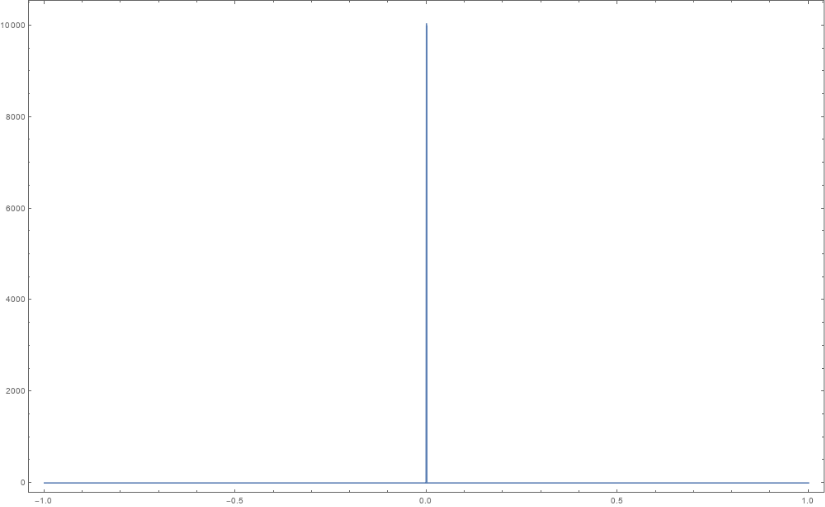
\includegraphics[scale=0.5]{delta-distribution.png}
	\caption{A Plot of $\delta(x)$}
\end{figure}
We can interpret \ref{del2} as saying "the area of the delta distribution is always 1".
\begin{equation}
f(x)\delta(x - a ) = f(a)
\end{equation}
We can combine these to get,
\begin{equation}
\int_{- \infty}^{+ \infty} \delta(x-a) f(x) dx = f(a)
\end{equation}
\subsubsection{A few interesting properties}
\begin{equation}
\delta(kx) = \frac{1}{|k|}\delta(x)
\end{equation}
\begin{equation}
\frac{d}{dx}(\delta(x)) = -\delta(x)
\end{equation}
where k is a constant
\begin{equation}
\frac{d \theta}{dx} = \delta(x)
\end{equation}
Where $\theta$ is the step function defined as,
\begin{equation}
\theta(x)= 
\begin{cases}
1, & \text{if } x > 0\\
o,              & \text{if } x \leq 0
\end{cases}
\end{equation}

\subsection{The Three-Dimensional Dirac Delta Function}
We generalize (\ref{deltadef}) to three dimensions,
\begin{equation}
\delta^{3}(\vec{r} - \vec{a}) = \delta(x-a_{x})\delta(y-a_{y})\delta(z-a_{z})
\end{equation}
\begin{equation}
\int_{- \infty}^{+ \infty} \delta^{3}(\vec{r} - \vec{a}) dV = 1
\end{equation}
We can also define the three-dimensional delta function as
\begin{equation}
\delta^{3}(\boldscriptr) = \frac{1}{4 \pi} \left[\nabla \cdot \left( \frac{\hat{\boldscriptr}}{{\scriptr	}^{2}}\right)\right]
\end{equation}
Since,
$$\nabla \left(\frac{1}{\scriptr}\right) = -\frac{\hat{\boldscriptr}}{\scriptr^{2}}$$
We can rewrite as,
\begin{equation}
\delta^{3}(\boldscriptr) = -\frac{1}{4 \pi} \left[\nabla^{2}  \left( \frac{1}{\scriptr}\right)\right]
\end{equation}
\subsection{Integral representation}
We have the relationship for the Fourrier transform,
\begin{equation}
F(x) = \int f(t) e^{-ixt} dt
\end{equation}
and it's inverese
\begin{equation}
f(t) = \frac{1}{2 \pi} \int F(x) e^{ixt} dx
\end{equation}
Plugging in Eq. into Eq. we find that 
\begin{equation}
	F(y) = \frac{1}{2 \pi} \int_{-\infty}^{\infty} F(x) dx \int_{-\infty}^{\infty}e^{i(x-y)t} dt
\end{equation}	
Now, invoking the definig property of the Delta function,
\begin{equation}
F(y) = \int_{-\infty}^{\infty} F(x) \delta(x-y) dx
\end{equation}
Comparing and we find that,
\begin{tcolorbox}
\begin{equation}
\delta(x-y) = \frac{1}{2 \pi} \int_{-\infty}^{\infty} e^{i(x-y)t} dt
\end{equation}
\end{tcolorbox}
\section{Complex Analysis}
\subsection{Complex Differentiation}
We call a function to \textbf{holomorphic} if it is differentiable in its domain.
\subsection{Contour Integrals}
\subsection{Cauchy-Goursat Theorem}
\subsection{Cauchy's Integral Formula}

\subsection{A few important relations}
\subsubsection{Cauchy-Riemann Equations}
\subsubsection{Laplace Equation}
\section{Gaussian Integrals}
In this section we'll try to solve integrals of the form
\begin{equation}
I_{0} (\alpha) = \int_{-\infty}^{\infty} e^{-\alpha x^{2}} dx \ \forall \ \alpha > 0
\end{equation}
We can't directly integrate it, so we consider
\begin{equation}
I^{2}_{0}(\alpha) = \int_{-\infty}^{\infty} e^{-\alpha y^{2}} dy\int_{-\infty}^{\infty} e^{-\alpha x^{2}} dx = \int_{-\infty}^{\infty}\int_{-\infty}^{\infty}e^{-\alpha (x^{2} + y^{2})} dxdy
\end{equation}
Switching to polar coordinates in the x-y plane,
\begin{equation}
I^{2}_{0}(\alpha) = \int_{0}^{\infty} \int_{0}^{2 \pi} e^{-\alpha \rho^{2}} d \rho \ d\phi = \frac{\pi}{\alpha}
\end{equation}
Therefore,
\begin{equation}
	I_{0}(\alpha) = \sqrt{\frac{\pi}{\alpha}}
\end{equation}
\subsection{Special Cases}
By differentiating w.r.t $\alpha$ we can get all integrals of the form:
\begin{equation}
I_{2n} (\alpha) = \int_{-\infty}^{\infty} x^{2n} e^{-\alpha x^{2}} dx
\end{equation}
For example,
$$I_{2}(\alpha) = \int_{-\infty}^{\infty} x^{2n} e^{-\alpha x^{2}} dx = -\frac{\partial }{\partial \alpha} \int_{-\infty}^{\infty} e^{-\alpha x^{2}} dx$$
$$I_{2}(\alpha) = \frac{\partial }{\partial \alpha} I_{0}(\alpha) = \frac{1}{2 \alpha} \sqrt{\frac{\pi}{\alpha}}$$
The integrals $I_{2n+1}(\alpha)$ vanish because they are integrals of odd functions over an even internval ($-\infty \text{ to } \infty$).
\\ \textbf{Note:} The integrals discussed so far are valid even if $\alpha \in \mathbb{C}$
Next we'll consider,
\begin{equation}
I_{0}(\alpha, \beta) = \int_{- \infty}^{\infty} e^{-\alpha x^{2} + \beta x} dx
\end{equation}
We can simplify this to be,
$$I_{0}(\alpha, \beta) = e^{\beta^{2}/ 4 \alpha} \int_{- \infty}^{\infty} e^{\alpha{(x - \beta / 2 \alpha)}^{2}} dx = e^{\beta^{2}/ 4 \alpha} \sqrt{\frac{\pi}{\alpha}}$$
This holds even if $\alpha, \beta \in \mathbb{C} : Re(\alpha) > 0$. A corollary of the previous equation,
$$\int_{0}^{\infty} e^{-\alpha r} dr = \frac{1}{\alpha}$$
if we operate on this with, ${(-d/d \alpha)}^{n}$ , we get:
$$\int_{0}^{\infty} r^{n} e^{-\alpha r} dr = \frac{n!}{\alpha^{n+1}}$$
\subsection{Gamma function}
If we consider this integral with $\alpha = 1$ and $n$ replaced with $z-1$, where $z$ is an abitrary complex number. This lead us to the Gamma function, which is defined as:
\begin{equation}
\Gamma (z) = \int^{0}_{\infty} r^{z-1} e^{-r} dr = (z-1)! \ \forall \ z > 0 \in \mathbb{R}
\end{equation}
\section{The $i \epsilon$ Prescription}
We will now derive and interpret the formula:
\begin{equation}
\frac{1}{x \mp i \epsilon} = \mathscr{P} \frac{1}{x} \pm \pi \delta (x)
\end{equation}
where $\epsilon \rightarrow 0$ is a positive infinitesimally small quantity. Now we'll consider the integral
\begin{equation}
	I = \lim_{\epsilon \rightarrow 0} \int_{- \infty}^{\infty} \frac{f(x)}{x - i \epsilon} dx
\end{equation}

$$	I = \lim_{\epsilon^{'} \rightarrow 0} \left[ \int_{- \infty}^{\epsilon^{'}} \frac{f(x)}{x} dx + \int_{- \infty}^{\epsilon^{'}} \frac{f(x)}{x} dx + i \pi f(0)\right]$$
\begin{equation}
I =   \mathscr{P}\int_{- \infty}^{\infty} \frac{f(x)}{x} dx + i \pi f(0)
\end{equation}
\begin{equation}
\frac{1}{(x-a)\mp i \epsilon} = \mathscr{P}\frac{1}{(x-a)}\pm i \pi \delta(x-a)
\end{equation}
\section{Permutation Functions}
\subsection{Kronecker delta}
It simply has the ‘function’ of ‘renaming’ an index:
$$\delta^{\mu}_{\nu} x^{\nu} = x^{\mu}$$
it is in a sense simply the identity matrix. Or it is sometimes defined as:
\begin{equation}
\delta_{ij} = \begin{cases}
1 \ \text{if } i = j \\
0 \ \text{if } i \neq j\\
\end{cases}
\end{equation}
\subsection{Levi-Civita Pseudotensor}
\label{Levi}
The Levi-Civita Pseudotensor i.e. Tensor density is a completely anti-symmetric i.e. $\epsilon_{ijk} = -\epsilon_{jik} = -\epsilon_{ikj} = -\epsilon_{kji}$, we define it as:
\begin{equation}
\epsilon_{ijk} = \begin{cases}
1 \ \text{if } ijk \text{ is an even permuation of } 123\\
-1 \ \text{if } ijk \text{ is an odd permuation of } 123\\
0  \text{ if two indices are equal}\\
\end{cases}
\end{equation}
\subsubsection{Identities}
\begin{equation}
\epsilon_{\alpha \beta \nu}\epsilon_{\alpha \beta \sigma} = \delta_{\mu \rho} \delta_{\nu \sigma} - \delta_{\mu \sigma}\delta_{\nu \rho} 
\end{equation}
From this it follows that,
\begin{equation}
\epsilon_{\alpha \beta \nu}\epsilon_{\alpha \beta \sigma} = 2\delta_{\nu \sigma}
\end{equation}
and
\begin{equation}
\epsilon_{\alpha \beta \gamma}\epsilon_{\alpha \beta \gamma} = 6
\end{equation}
\section{Tensors}
\subsection{Vector Transformation Rules}
The rules:
\begin{itemize}
	\item For basis vectors forward transformations brings us from old to new coordinate systems and backward brings us from new to old.
	\item However, with vector components it's the opposite.\\
\end{itemize}

Suppose we have a vector $\vec{v}$ in a basis $\vec{e}_j$. We now transform it to a basis $\tilde{\vec{e}}_i$ where it becomes $\tilde{v}$. We call the forward transformation as $F_{ij}$ and the backward as $B_{ij}$ which we define as:
$$\tilde{\vec{e}}_j = \sum_{i = 1}^{n} F_{ij} \vec{e}_i$$
$$\vec{e}_j = \sum_{i = 1}^{n} B_{ij} \tilde{\vec{e}}_i$$
We can try to derive the statements made previously,
$$\vec{v} = \sum_{j = 1}^{n} v_{j}\vec{e}_j = \sum_{i = 1}^{n} \tilde{v}_{i}\tilde{\vec{e}}_i$$
$$\vec{v} = \sum_{j = 1}^{n} v_{j}\vec{e}_j = \sum_{j = 1}^{n} {v}_{j}(\sum_{i=1}^{n} B_{ij} \tilde{\vec{e}}_i) =  \sum_{i = 1}^{n} \sum_{j = 1}^{n} (B_{ij} {v}_{j}) \tilde{\vec{e}}_i$$
Thus,
\begin{equation}
	\tilde{v}_i = \sum_{j = 1}^{n} B_{ij} {v}_{j}
\end{equation}
Similarly,
$$\vec{v} = \sum_{j = 1}^{n} v_{j}\vec{e}_j = \sum_{i = 1}^{n} \tilde{v}_{i}\tilde{\vec{e}}_i$$
$$\vec{v} = \sum_{j = 1}^{n} \tilde{v}_{j}\tilde{\vec{e}}_j = \sum_{j = 1}^{n} \tilde{v}_{j}(\sum_{i = 1}^{n} F_{ij} \vec{e}_i) =  \sum_{i = 1}^{n} \sum_{j = 1}^{n} (F_{ij} \tilde{v}_{j}) {\vec{e}}_i$$
Thus,
\begin{equation}
	{v}_i = \sum_{j = 1}^{n} F_{ij} \tilde{v}_{j}
\end{equation}
Now because vector components beehave contrary to the basis vectors, they are said to be \textit{\textbf{"Contravariant"}}
\subsection{Index Notation}
\subsubsection{Einstein Notation i.e. Summing convention}
Let us consider the sum\footnote{Mind you there are no exponents there.},
$$x_{i} = \sum_{j}^{n}\Lambda_{ij}\mathcal{X}^{j}$$
Is the same as,
$$x_{i} = \Lambda_{ij}\mathcal{X}^{j}$$ 
Here, we define $i$ to be the free index and $j$ to be the summing index or the dummy index that is repeated to signify so.
\subsubsection{Index Convention}
When we sum from $1$ to $3$ we use the symbols $i,j$ and $k$ i.e. the English alphabet to signify that we are only considering dimnesions that are spatial/that are not a timme dimension. However, when we use the symbols $\nu$ and $\mu$ i.e. Greek alphabets we are summing from 0 to 3, we also include the temporal dimension according to the tradition of special relativity in which we name components as $\{x^{0}, x^{1}, x^{2}, x^{3}\} = \{t, x, y, z\}$ in the Cartesian framework.

\subsection{Covectors}
\begin{itemize}
	\item Covectors can be thought of as row vector or as functions that act on Vectors such that any covector $\alpha : \mathbb{V} \rightarrow \mathbb{R}$
	\item Covectors are linear maps i.e. $ \beta ( \alpha ) \vec{v} = \beta \alpha \vec{v}$ and $(\beta + \alpha ) \vec{v} = \alpha \vec{v} + \beta \vec{v}$
	\item Covectors are elements of a Dual vector space $\mathbb{V}^*$ which has different rules for addition and scaling i.e. scalar multiplication
	\item You visualize covectors to be some sort of gridline on your vector space such that applying a covector to a vector is equivalent to projecting the vector along the gridline
	\item Covectors are invariant but their components are not
	\item The covectors that form the basis for the set of all covectors is called the \textit{\textbf{"Dual Basis"}}, because they are a basis for the Dual Space $\mathbb{V}^*$ i.e. any covector can be expressed as the linear combination of the dual basis
	\item However we are free to choose a dual basis
	\item For covector components, forward transformation brings us from old to new and backwards vice versa
	\item We can flip between row and column vectors for an orthonormal basis
	\item Vector components are measured by counting how many are used in the construction of a vector, but covector components are measured by counting the number of covector lines that the basis vector pierces
	\item The covector basis transforms contravariantly compared to the basis and it's components transform covariantly according to the basis 
\end{itemize}


\subsubsection{Contravariant Components}
We denote contravariant components using the symbols
$$A^i$$
and their basis like
$$\overrightarrow{e}_i$$
\subsubsection{Covariant Components}
We denote convariant components using the symbols
$$A_i$$
and their basis like
$${\overrightarrow{e}}^i$$
\subsubsection{Relationship Between the Two Types of Components}

$$|\overrightarrow{e}^1| = \frac{1}{|\overrightarrow{e}_1|\cos(\theta_1)}$$
and,
$$|\overrightarrow{e}_1| = \frac{1}{|\overrightarrow{e}^1|\cos(\theta_1)}$$
Or with 3 components we have:
Since both types of components represent the same vector (as in same magnitude) only inn  different bases, we can write
$$\overrightarrow{A} = A^{i}\overrightarrow{e}_i = A_{i}\overrightarrow{e}^i$$
\subsubsection{Using Cramer's Method to find Components}

\subsection{Metric Tensor}
\begin{itemize}
	\item Pythagoras' theorem is a lie for non-orthonormal bases
	\item The metric Tensor is Tensor that helps us compute lengths and angles
	\item For two dimensions it can be written as:
\end{itemize}
$$\textit{g}_{ij} = \begin{bmatrix}
	e_{1}e_{1} & e_{1}e_{2} \\
	e_{2}e_{1} & e_{2}e_{2} 
\end{bmatrix}$$
\begin{itemize}
	\item Or more abstractly
\end{itemize}
$$\textit{g}_{ij} = e_{i}e_{j}$$
\begin{itemize}
	\item The dot product between two vectors can be written as
\end{itemize}
$$||\vec{v}|| ||\vec{w}||\cos{\theta} = v^{i}w^{j}\textit{g}_{ij}$$
\begin{itemize}
	\item we can see how this allows us to compute angles as well
	\item To transform the components of the Metric Tensor we have to apply the transformation twice i.e.$\tilde{g}_{\rho \sigma} = \mathbb{F}^{\mu}_{\rho} \mathbb{F}^{\nu}_{\sigma}\tilde{g}_{\mu \nu}$ or $g_{\rho \sigma} = \mathbb{B}^{\mu}_{\rho} \mathbb{B}^{\nu}_{\sigma}\tilde{g}_{\mu \nu}$
\end{itemize}

\subsection{Tensor Products}

\subsection{Definition of a Tensor}


\chapter{Toy Models}
\section{Time-Dependent Schrodinger Equation}
\section{Time-Independent Schrodinger Equation}
\section{Stationary States}
\section{The Infinite Square Well}
\section{Harmonic Oscillator}
\section{Free Particle}
\section{Delta-Function Potential}
\section{Finite Square Well}
\section{Wave-Packets}
\chapter{Systems with N degrees of freedom}
\section{Schrodinger Equation in 3 Dimensions}
\section{The Hydrogen Atom}
\section{N Particles in One Dimension}
\section{More Particles in More Dimensions}
\section{Identical Particles}
\section{Two-Particle Systems}
\section{Atoms}
\section{Solids}
\section{Quantum Statistical Mechanics}
\chapter{The Second Chapter}
\chapter{Hydrogen Atom}


\chapter{Approximations}
\chapter{Pertubation Theory}
\section{Non-Degenerate Perturbation Theory}
\subsection{General Formulation}
Suppose we have solved the time-independent Schrodinger wave equation for a given potential (in this case, an infinite potential square well)
\begin{equation}
H^0\psi_{n}^0=E^{0}_{n}\psi_{n}^0
\end{equation}
and obtaining a complete set of orthonormal eigenfunctions $\psi_{n}^0$,
\begin{equation}
\bra{\psi_{n}^0}{\psi_{m}^0}\rangle=\delta_{nm}
\end{equation}
and the corresponding eigenvalues $E^0_n$. If we perturb the potential slightly in the potential well and try to solve for the new eigenvalues and eigenfunctions, 
\begin{equation}
H\psi_n=E_n\psi_n
\end{equation}
Here, we use perturbation theory to get approximate solutions to the perturbed problem by building on the exact solutions of the unperturbed case.\\
To begin with, we write the perturbed/new Hamiltonian as the sum of two terms,
\begin{equation}
H=H^0+\lambda H'
\end{equation}
Where H' is the perturbation. We take $\lambda$ to be a small number, and the $H$ will be the true, exact Hamiltonian. Writing $\psi_n$ and $E_n$ as a power series in $\lambda$, we get,
\begin{gather}
\psi_{n}=\psi_{n}^0 + \lambda \psi_{n}^1 + \lambda^2 \psi_{n}^2+... \\
E_n= E^0_n + \lambda E^1_n + \lambda^2 E^2_n+...
\end{gather}
Here $E^1_n$ is the first-order correction to the $n^th$ eigenvalue, and $\psi_{n}^1$ is the first-order correction to the $n^th$ eigenfunction. $E^2_n$ and $\psi_{n}^2$ are the second-order corrections to the eigenvalues and eigenfunctions, and so on. Plugging in Equations (4),(5) and (6) in Equation (3) gives us,
\begin{multline}
(H^0+\lambda H')[\psi_{n}^0 + \lambda \psi_{n}^1 + \lambda^2 \psi_{n}^2+... ]=\\( E^0_n + \lambda E^1_n + \lambda^2 E^2_n+...)[\psi_{n}^0 + \lambda \psi_{n}^1 + \lambda^2 \psi_{n}^2+...]
\end{multline}
We can rewrite Equation (7) by collecting like powers of $\lambda$ in the form,
\begin{multline*}
H^0\psi^0 + \lambda(H^0\psi^1_n+H'\psi_n^0) + \lambda^2(H^0\psi^2_n+H'\psi^1_n)+...\\E^0_n\psi^0 + \lambda(E^0_n\psi^1_n+E^1_n\psi_n^0) + \lambda^2(E^0_n\psi^2_n+E_n^1\psi^1_n+E^2_n\psi^0_n)+...
\end{multline*} 
We can get the first order ($\lambda^1$) equation from Equation (7),
\begin{equation}
H^0\psi_{n}^1+H'\psi^0_n=E^0_n\psi^1_n+E^0_n+\psi_n^0
\end{equation}
And the second order ($\lambda^2$),
\begin{equation}
H^0\psi_{n}^2+H'\psi^1_n=E^0_n\psi^2_n+E^1_n\psi^1_n+E^2_n\psi^0_n
\end{equation}
And this can be done for higher powers of $\lambda$ as well.

\subsection{First order perturbation theory}
If we take the inner product of Equation (8), with $\psi^0_n$,
\begin{equation}
\langle\psi^0_n\vert H^0\psi^1_n\rangle + \langle\psi^0_n\vert H'\psi^0_n\rangle=E^0_n\langle\psi^0_n\vert\psi^1_n\rangle +E^1_0\langle\psi^0_n\vert\psi^0_n\rangle
\end{equation}
Because of the useful property of $H^0$ to be Hermitian, hence Equation (10) becomes,
\begin{equation}
\langle\psi^0_n\vert H^0\psi^1_n\rangle=\langle H^0\psi^0_n\vert \psi^1_n\rangle=E^0_n\langle\psi^0_n\vert\psi^1_n\rangle=\langle E^0_n\psi^0_n\vert\psi^1_n\rangle
\end{equation}
And hence the terms in Equation (10) cancel out and the property $\langle\psi^0_n\vert\psi^0_n\rangle=1$ give the equation,
\begin{equation}
E^1_n=\langle\psi_n^0\vert H'\vert\psi^0_n\rangle
\end{equation}
This is a fundamental result in first-order perturbation theory, and it states that first-order correction to energy is the expectation value of the pertubation in the unperturbed state.

Now to get the first-order correction to the wave function, we rewrite Equation (8),
\begin{equation}
(H^0-E^0_n)\psi^1_n=-(H'E^1_n)\psi^0_n
\end{equation}
The right side is a known fucntion, so this amounts to an inhomogenious differential equation for $\psi^!_n$. The unpertubed wave functions constitute a complete set, so $\psi^1_n$ can be writtten as a linear combination of them,
\begin{equation}
\psi^1_n=\sum_{m\neq n}c^{(n)}_m\psi^0_m
\end{equation}
We know that $\psi^0_m$ satisfies the unpertubed Schrodinger wave equation, so we have,
\begin{equation}
\sum_{m\neq n}^{}(E^0_m-E^0_n)c^{(n)}_m\psi^0_m=-(H'-E^1_n)\psi^0_n
\end{equation}

Taking the inner product with $\psi^0_l$,
\begin{equation}
\sum_{m\neg n}(E^0_m-E^0_n)c^{(n)}_m\braket{\psi^0_l}{\psi^0_m}=-\langle\psi^0_l\vert H' \vert \psi^0_n\rangle+E^1_n\braket{\psi^0_l}{\psi^0_n}
\end{equation}
If $l=n$, is zero, we then get,

\begin{equation}
E^0_m-E^0_n)c^{(n)}_l=-\langle\psi^0_l\vert H' \vert \psi^0_n\rangle
\end{equation}
Or that,
\begin{equation}
c^{(n)}_n=\frac{\langle\psi^0_m\vert H' \vert \psi^0_n\rangle}{E^0_n-E^0_m}
\end{equation}
So,
\begin{equation}
\psi^1_n=\sum_{m\neg n}\frac{\langle\psi^0_m\vert H' \vert \psi^0_n\rangle}{E^0_n-E^0_m}\psi^0_m
\end{equation}
Note that the perturbed energies are surprisingly accurate, while the wave functions are of poor accuracy.


\subsection{Second order perturbation theory}
We take the inner poduct of the second-order equation with $\psi^0_n$,
\begin{equation}
\braket{\psi^0_n}{H^0\psi^2_n}+\braket{\psi^0_n}{H'\psi^1_n}=E^0_n\braket{\psi^0_n}{\psi^2_n}+E^1_n\braket{\psi^0_n}{\psi^1_n}+ E^2_n\braket{\psi^0_n}{\psi^0_n}
\end{equation}
We exploit the Hermiticity of $H^0$,
\begin{equation}
\braket{\psi^0_n}{H^0\psi^2_n}=\braket{H^0\psi^2_n}{\psi^2_n}=E^0_n\braket{\psi^0_n}{psi^2_n}
\end{equation}
So the first term on the left cancels the first term on the right. Hence we get the formula for $E^2_n$ to be,
\begin{equation}
E^2_n=\langle\psi^0_n\vert H' \vert \psi^1_n\rangle - E^1_n\braket{\psi^0_n}{\psi^1_n}
\end{equation}
But,

\begin{equation}
\braket{\psi^0_n}{\psi^1_n}=\sum_{m\neq n}^{}c^{(n)}_m\braket{\psi^0_n}{\psi^0_m}=0
\end{equation}

so,
\begin{equation}
E^2_n=\langle\psi^0_n\vert H' \vert \psi^1_n\rangle=\sum_{m\neq n}^{}c^{(n)}_m\braket{\psi^0_n}{\psi^0_m}= \sum_{m\neq n}^{}c^{(n)}_m\frac{\langle\psi^0_m\vert H' \vert \psi^0_n\rangle \langle\psi^0_m\vert H' \vert \psi^0_n\rangle}{E^0_n-E^0_m}
\end{equation}
Therefore,
\begin{equation}
E^2_n= \sum_{m\neq n}^{}c^{(n)}_m\frac{\vert\langle\psi^0_m\vert H' \vert \psi^0_n\rangle\vert^2}{E^0_n-E^0_m}
\end{equation}
This is the fundamental result of second order perturbation theory.

\section{Degenerate Perturbation Theory}
\subsection{Motivation}
If two or more distinct states, take $\psi^0_a$ and $\psi^0_b$ share the same energy, ordinary perturbation theory fails since Equation (25) blows up. So hence we need to obtain a different way to handle the problem.

\subsection{Twofold Degeneracy}
Suppose,
\begin{align*}
H^0\psi^0_a=E^0\psi^0_a\\
H^0\psi^0_b=E^0\psi^0_b\\
\braket{\psi^0_a}{\psi^0_b=0}
\end{align*}
And note that any of linear combinations of these states,
\begin{equation}
\psi^0=\alpha\psi^0_a+\beta\psi^0_b
\end{equation}
is still an eigenstate of $H^0$, with the same eigenvalue $E^0$,
\begin{equation}
H^0\psi^0=E^0\psi^0
\end{equation}	 
When $H$ is perturbed, it breaks the degeneracy. When we increase $\lambda$, the common unperturbed energy $E^0$ splits into two. When we take away the perturbation, the upper state redyces to one linear combination of $\psi^0_a$ and $\psi^0_b$, and the lower state reduces to some other linear combination. We need to figure out the good linear combinations.\\
Now writing the good unperturbed states in general form, keeping $\alpha$ and $\beta$ adjustable and solving the Schrodinger equation,
\begin{equation}
H\psi=E\psi
\end{equation}
With $H=H^0+\lambda H'$ and,
\begin{align}
E=E^0+\lambda E^1 + \lambda^2 E^2 +...\\
\psi=\psi^0+\lambda\psi^1+\lambda^2\psi^2+...
\end{align} 
Plugging these into Equation (28) and collecting like powers of $\lambda$, as before, we find,
\begin{equation}
H^0\psi^0+\lambda(H\psi^0+H^0\psi^1)+...=E^0\psi^0+\lambda(E^1\psi^0+E^0\psi^1)+...
\end{equation}
But $H^0\psi^0=E^0\psi^0$, so the first term cancel; at order $\lambda^1$ we have,
\begin{equation}
H\psi^0+H^0\psi^1=E^1\psi^0+E^0\psi^1
\end{equation}
Taking inner product with $\psi^0_a$,
\begin{equation}
\langle\psi^0_a\vert H^0 \vert \psi^1\rangle+ \langle\psi^0_a\vert H' \vert \psi^0\rangle=E^0\braket{\psi^0_a}{\psi^1} + E^1\braket{\psi^0_a}{\psi^0}
\end{equation}
Because $H^0$ is Hermitian, the first term on the left cancels the term on the right. Putting this in Equation (26), we get,
\begin{equation}
\alpha \langle\psi^0_a\vert H' \vert \psi^0_a\rangle=\beta \langle\psi^0_a\vert H' \vert \psi^0_b\rangle=\alpha E^1
\end{equation}
Or in a more compact form,
\begin{equation}
\alpha W_{aa}+\beta W_{ab}=\alpha E^1
\end{equation}
Where,
\begin{equation*}
W_{ab}= langle\psi^0_a\vert H' \vert \psi^0_b\rangle
\end{equation*}
Similarly, the inner product with $\psi^0_b$ gives us,
\begin{equation}
\alpha W_{ba}+\beta W_{bb}=\beta E^1
\end{equation}
Now using Equation (35) and (36),
\begin{equation}
\alpha[W_{ab}W_{ba}-(E^1-W_{aa}))(E^1-W_{bb})]=0
\end{equation}
When $\alpha\neq 0$,
\begin{equation}
(E^1)^2-E^1(W_{aa}+W{bb})+(W_{aa}W_{bb}-W_{ab}W_{ba})=0
\end{equation}
Using the quadratic formula and knowing that $W_{ba}=W^*_{ab}$,
\begin{equation}
E^1_\pm=\frac{1}{2}\left[W_{aa}+W_bb\pm\sqrt{(W_{aa}-W_{bb})^2+4\vert W_{ab}\vert^2}\right]
\end{equation}
This is the fundamental result of degenerate pertubration theory, the two roots correspond to the two perturbed energies.\\
Note that when $\alpha=0$, we get the nondegenerate perturbation theory (since $\beta=1$).

\subsection{Higher-Order Degeneracy}
We start by rewriting Equations (35) and(36) in matrix form,
\begin{gather}
\begin{pmatrix}
W_{aa} & W_{ab}\\
W_{ba} & W_{bb}
\end{pmatrix}
\begin{pmatrix}
\alpha\\
\beta
\end{pmatrix}
= E^1
\begin{pmatrix}
\alpha\\
\beta
\end{pmatrix}
\end{gather}
The $E^1$s are the eigenvalues of the $W$-matrix, Equation (38) being the characteristic equation for this matrix and the good linear combinations of the unperturbed states are the eigenvectors of $W$. For $n$-fold degeneracy, we look for the eigenvalues of the $n\cross n$ matrix,
\begin{equation}
W_{ij}=\langle \psi^0_i\vert H' \vert \psi^0_j\rangle
\end{equation}
\subsection{Lamb Shift}
An interesting feature of the fine structure formula is that it depends only on $j$ and not $l$, moreover in general two different values of $l$ share the same energy. For example, the $2S_{1/2} ()$ and $2P_{1/2} ()$ states should remain perfectly degenerate. However in 1947 Lamb and Retherford performed an experiment that displayed something to the contrary. The $S$ state is slightly higher in energy than the $p$ state. The explanation of this "Lamb" shift was later explained by Bethe, Feynman, Schwinger and Tomonaga (the founders of QED) as a corollary of the electromagnetic field itself being quantised.  Sharply in contrast to the hyperfine structure of Hydrogen, the Lamb shift is a completely novel i.e. non-classical (as the hyperfine structure is explained through Coulomb's law and the Biot-Savart Law) phenomena. It arises from a radiative correction in Quantum Electrodynamics to which classical theories are mute. In Feynman lingo, this arises from loop corrections as potrayed below.
\begin{figure}[h]
	\centering
	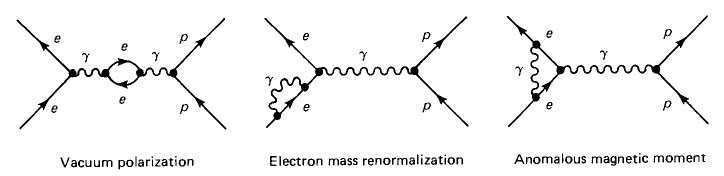
\includegraphics[width=0.6\linewidth, height=0.3\linewidth]{feyn-loop.png}
	\caption{Different kinds of radiative corrections}
\end{figure}
Naively,
\begin{enumerate}
	\item the first diagram describes pair-production in the neighbhorhood of a nucleus, leading to a partial screening effect of the proton's charge;
	\item the second diagram reflects the fact that the electromagnetic field has a non-zero ground state
	\item the third diagram leads to a tiny modification of the electron's magnetic dipole moment (an addition of $a + \alpha/2\pi = 1.00116$)
\end{enumerate}
We shall not discuss the results in depth but rather consider two exemplary cases:\\
For $ l = 0$,
\begin{equation}
\Delta E_{Lamb} = \alpha^{5}mc^{2}\frac{1}{4n^{3}}\left[k(n,0)\right]
\end{equation}
Where $k(n,0)$ is a numerical factor defined as:
$$k(n,0) = \begin{cases}
12.7, & \text{if } n = 1\\
13.2,              & \text{if } n \rightarrow \infty
\end{cases} $$
For $ l = 0$ and $j = l \pm \frac{1}{2}$,
\begin{equation}
\Delta E_{Lamb} = \alpha^{5}mc^{2}\frac{1}{4n^{3}}\left[ k(n,0) \pm \frac{1}{\pi (l + \frac{1}{2}) (l + \frac{1}{2})} \right]
\end{equation}
Here, $k(n,l)$ is a very small number $(< 0.05)$ which varies a little with it's arguments.\\
The Lamb shift is tiny except for the case $l=0$, for which it amounts to about $10 \% $ of the fine structure. However, since it depends on $l$, it lifts the degeneracy of the pairs of states with common $n$ and $j$ and in particular it splits $2 S_{1/2}$ and $2 P_{1/2}$.
\section{The Zeeman Effect}
When an atom is placed in a uniform magnetic field $B_{Ext.}$, the energy levels are shifted, this is known as the Zeeman effect. For the case of a single electron, the shift is:
\begin{equation}\label{zeeman_def}
H^{'}_{Z} = -(\mu_{l} + \mu_{s}).B_{Ext.}
\end{equation}
Where,
\begin{equation}
\mu_{s} = -\frac{e}{m_{e}}S
\end{equation}
is the magnetic dipole moment associated with electron spin, and
\begin{equation}
\mu_{l} = -\frac{e}{2m_{e}}L
\end{equation}
is the dipole moment associated with orbital motion. The gyromagnetic ratio in this case is simply classical i.e. $q/2m$, it is only for spin that we have an extra factor of 2. We now rewrite (\ref{zeeman_def}) as:
\begin{equation}
H^{'}_{Z} = \frac{e}{2m_{e}}(L + 2S).B_{Ext.}
\end{equation}
The nature of the Zeeman splitting depnds on the strength of the external field vs. the internal one that gives rise to spin-orbit/spin-spin coupling. This table provides a short review of the different cases:
\begin{center}
	\begin{tabularx}{0.9\textwidth} { 
			| >{\centering\arraybackslash}X 
			| >{\centering\arraybackslash}X 
			| >{\centering\arraybackslash}X | }
		\hline
		\textbf{Case} & \textbf{Name} & \textbf{Comments} \\
		\hline
		$B_{Ext.} >> B_{Int.}$  & Strong-Field Zeeman Effect  & Zeeman effect dominates; fine structure becomes the perturbation  \\
		\hline
		$B_{Ext.} << B_{Int.}$  & Weak-Field Zeeman Effect  & Fine structure dominates; $H^{'}_{z}$ can be treated as a small perturbation   \\
		\hline
		$B_{Ext.} = B_{Int.}$  & Intermediate Zeeman Effect  & Both the fields are equal in strength thus we would need elements of degenerate peturbation theory and will need to diagonlize the necessary portion of the Hamiltonian "by hand" \\
		\hline
	\end{tabularx}
\end{center}
In the next few sections we'll explore all of them in depth.
\subsection{Weak-Field Zeeman Effect}
Here the fine structure dominates, thus the conserved quantum numbers are $n$, $l$, $j$ and $m_{j}$, but not $m_{l}$ and $m_{s}$ due to the spin-orbit coupling L and S are not separately conserved. Generally speaking, in this problem we have a perturbation pile on top of a perturbation. Thus, the conserved quantum number are those appropriate to the dominant . In first order perturbation theory, the Zeeman correction to energy is,
\begin{equation}
E^{1}_{Z} = \expval{H^{'}_{Z}}{nlj m_{j}} = \frac{e}{2m}B_{Ext.} \expval{L + 2S}
\end{equation} 
Now to figure out $\expval{L + 2S}$, we know that $L + 2S = J + S$, this doesn't immediately tell us the expectation value of $S$ but we can figure it out as by understanding that $J = L + S$ is conserved and that the time average of $S$ is simply it's projection along $J$:
\begin{equation}
S_{Ave} = \frac{(S.J)}{J}J
\end{equation}
But, $L = J - S$, so  $L^{2} = J^{2} + S^{2} - 2 J.S$, hence:
\begin{equation}
S.J = \frac{1}{2}(J^{2} + S^{2} - 2 J.S) = \frac{\hbar^{2}}{2}[j(j+1)+ s(s+1)-l(l+1)]
\end{equation}
from which it follows that,
\begin{equation}
\expval{L + 2S} = \expval{\left(1 + \frac{S.J}{J^{2}}J\right)} = \left[1 + \frac{j(j+1)-l(l+1) + 3/4}{2j(j+1)}\right]\expval{J}
\end{equation}
The term in the square brackets is called the Lande g-factor, denoted by $g_{j}$. Now, if we choose $B_{z}$ to lie along $B_{Ext.}$, then:
\begin{equation}
E^{1}_{Z} = \mu_{B} g_{j} B_{Ext.} m_{j}
\end{equation}
where,
$$\mu_{B} = \frac{e \hbar}{2m} = 5.788 \times 10^{-5} \ eVT^{-1}$$
is the so called Bohr magneton. The total energy is the sum of the fine-structure part and the Zeeman contribution, in the ground state i.e. $n = 1, l = 0, j = 1/2$ and therefore, $g_{J} = 2$, it splits into two levels:
\begin{equation}
-13.6 \ eV(1 + \alpha^{2}/4) \pm \mu_{B} B_{Ext.}
\end{equation}
with different signs for different $m_{j}$'s this is plotted below.
\begin{figure}[h]
	\centering
	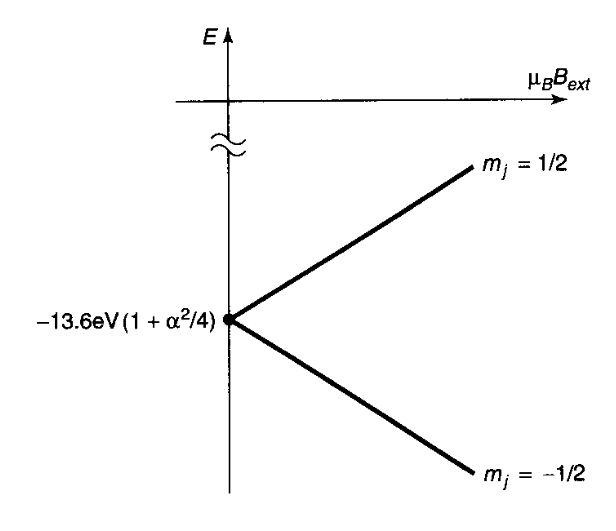
\includegraphics[width=0.6\linewidth, height=0.5\linewidth]{strong-split.png}
	\caption{Weak-field Zeeman splitting of the ground state of hydrogen; the upper line has a slope of $1$ and the lower line a slope of $-1$}
\end{figure}
\begin{figure}[h]
	\centering
	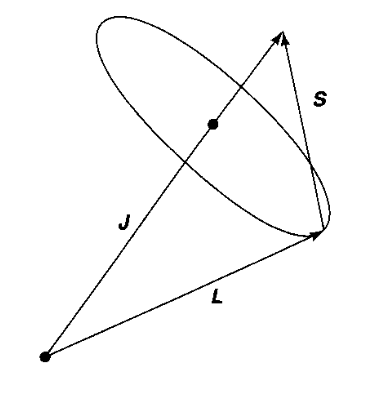
\includegraphics[width=0.6\linewidth, height=0.5\linewidth]{weak-split.png}
	\caption{In the presence of spin-orbit coupling, $L$ and $S$ are not separately conserved, they precess about the fixed total angular momentum $J$}
\end{figure}
\subsection{Strong-Field Zeeman Effect}
In this case, the Zeeman effect is often referred to as the "Paschen-Back" effect. The conserved quantum numbers are now but and because in the presence of an external torque, the total angular momentum is not conserved but the it's individual components are. The Zeeman Hamiltonian is,
\begin{equation}
H^{'}_{Z} =  \frac{e}{2m} B_{Ext.} (L_{z} + 2 S_{z})
\end{equation}
and the unperturbed energies are:
\begin{equation}
E_{nm_{l}m_{s}} = -\frac{13.6 \ eV}{n^{2}} + \mu_{B}B_{Ext.}(m_{l} + 2 m_{s})
\end{equation}
This would be our result if we ignore the fine structure completely. However, we need to take that into account as well. In first-order perturbation theory, the fine structure correction to these levels is:
\begin{equation}
E^{1}_{fs} = \expval{H^{'}_{r} + H^{'}_{so}}{n \ l \ m_{l} \ m_{s}}
\end{equation}
The relativistic contribution is the same as before for the spin-orbit term, we need
\begin{equation}
\expval{S.L} = \expval{S_{x}}\expval{L_{x}} + \expval{S_{y}}\expval{L_{y}} + \expval{S_{z}}\expval{L_{z}} = \hbar^{2}m_{l}m_{s}
\end{equation}
Here $\expval{S_{x}} = \expval{S_{y}} = \expval{L_{x}} = \expval{L_{y}} = 0$ for the eigenstates of $S_{z}$ and $L_{z}$. Putting it all together:
\begin{equation}
E^{1}_{fs} = \frac{13.6 \ eV}{n^{3}}\alpha^{2} \left(\frac{3}{4n} - \left[ \frac{l(l+1)-m_{l}m_{s}}{l(l+1/2)(l+1)}\right]\right)
\end{equation}
Th term in the square brackets is indeterminate for $l=0$, it's correct value in this case is 1. The total energy here is the sum of the Zeeman part and the fine structure contribution.
\subsection{Intermediate Zeeman Effect}
In this case, we must treat both the effects as perturbations to the Bohr Hamiltonian,
\begin{equation}
H^{'} = H^{'}_{Z} + H^{'}_{fs}
\end{equation}
In section we'll discuss the case $n = 2$, and use it as the basis for degerate perturbation theory. The states here are characterized by $l$, $j$ and $m_{j}$. We could use $l$,$m_{l}$,$m_{s}$ states but this makes the matrix elements of $H^{'}_{Z}$ easier to deal with but that of $H^{'}_{fs}$ difficult. Using the Clebsch-Gordan coefficients to express $\ket{j m_{j}}$ as a linear combination of $\ket{l m_{l}} \ket{s m_{s}}$ we have:
$$l = 0 = \begin{cases}
\psi_{1} & \ket{\frac{1}{2} \frac{1}{2}} = \ket{0 \ 0}\ket{\frac{1}{2}\frac{1}{2}}\\
\psi_{2} & \ket{\frac{1}{2} \frac{-1}{2}} = \ket{0 \ 0}\ket{\frac{1}{2}\frac{-1}{2}}
\end{cases} $$
$$l = 1 = \begin{cases}
\psi_{3} & \ket{\frac{3}{2} \frac{3}{2}} = \ket{1 \ 1}\ket{\frac{1}{2}\frac{1}{2}}\\
\psi_{4} & \ket{\frac{3}{2} \frac{-3}{2}} = \ket{1 \ -1}\ket{\frac{1}{2}\frac{-1}{2}}\\
\psi_{5} & \ket{\frac{3}{2} \frac{1}{2}} = \sqrt{2/3}\ket{1 \ 0}\ket{\frac{1}{2}\frac{1}{2}} + \sqrt{1/3}\ket{1 \ 1}\ket{\frac{1}{2}\frac{-1}{2}}\\
\psi_{6} & \ket{\frac{1}{2} \frac{1}{2}} = -\sqrt{1/3}\ket{1 \ 0}\ket{\frac{1}{2}\frac{1}{2}} + \sqrt{2/3}\ket{1 \ 1}\ket{\frac{1}{2}\frac{-1}{2}}\\
\psi_{7} & \ket{\frac{3}{2} \frac{-1}{2}} = \sqrt{1/3}\ket{1 \ -1}\ket{\frac{1}{2}\frac{1}{2}} + \sqrt{2/3}\ket{1 \ 0}\ket{\frac{1}{2}\frac{-1}{2}}\\
\psi_{8} & \ket{\frac{1}{2} \frac{-1}{2}} = -\sqrt{2/3}\ket{1 \ -1}\ket{\frac{1}{2}\frac{1}{2}} + \sqrt{1/3}\ket{1 \ 0}\ket{\frac{1}{2}\frac{-1}{2}}\\
\end{cases} $$
In this basis the matrix the non-zero elements of $H^{'}_{fs}$ are all on the diagonal and are given by the Bohr model. $H^{'}_{z}$ has four off diagonal elements. The complete matrix, W as we will see is more complicated but its eigenvalues are the same since they are independent of the chosen basis.
\begin{equation}
\begin{pmatrix}
5 \gamma - \beta & 0 & 0 & 0 & 0 & 0 & 0 & 0 \\
0 & 5 \gamma + \beta & 0 & 0 & 0 & 0 & 0 & 0\\
0 & 0 & \gamma - 2 \beta & 0 & 0 & 0 & 0 & 0\\
0 & 0 & 0 & \gamma + 2 \beta & 0 & 0 & 0 & 0\\
0 & 0 & 0 & 0 & \gamma - \frac{2}{3} \beta & \frac{\sqrt{2}}{3} \beta & 0 & 0\\
0 & 0 & 0 & 0 & \frac{\sqrt{2}}{3} \beta & 5 \gamma - \frac{1}{3} \beta & 0 & 0\\
0 & 0 & 0 & 0 & 0 & 0 & \gamma + \frac{2}{3} \beta & \frac{\sqrt{2}}{3} \beta\\
0 & 0 & 0 & 0 & 0 & 0 & \frac{\sqrt{2}}{3} \beta & 5 \gamma + \frac{1}{3} \beta
\end{pmatrix}
\end{equation}
Where,
$$\gamma = {(\alpha / 8)}^{2}13.6 \ eV$$
and,
$$\beta = \mu_{B}B_{Ext.}$$
The first four eigenvalues are already displayed along the diagonal. We only need to find the eigenvalues of the two  $2 \times 2$ blocks. The characteristic equation for the first one is given as:
\begin{equation}
\lambda^{2} - \lambda(6\gamma - \beta) + \left(5 \gamma^{2} - \frac{11}{3} \gamma \beta\right) = 0
\end{equation} 
and the quadratic formula gives the eigenvalues:
\begin{equation}
\lambda_{\pm} = 3 \gamma - (\beta /2) \pm \sqrt{4 \gamma^{2} + (2/3) \gamma \beta + (\beta^{2}/4)} 
\end{equation}
The eigenvalues of the second block are the same but with the sign of $\beta$ reversed. The eight energy levels are listed in the table and are plotted against in the figure (). In the zero field limit they reduce to the fine structure values. For the other cases, the splitting is seen clearly.
\begin{figure}[h]
	\centering
	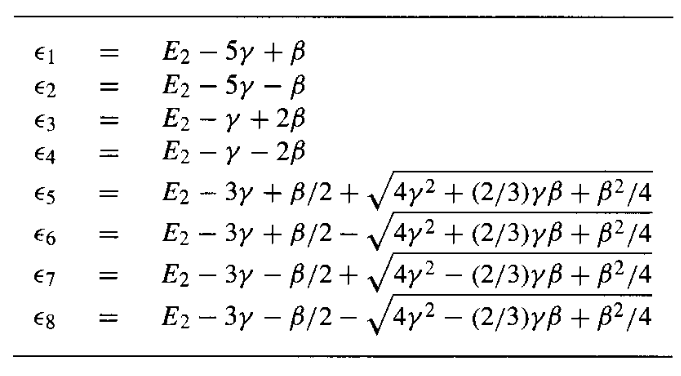
\includegraphics[width=0.6\linewidth, height=0.3\linewidth]{zee-table.png}
	\caption{Energy levels for the $n=2$ states of hydrogen, with fine structure and Zeeman splitting}
\end{figure}
\begin{figure}[h]
	\centering
	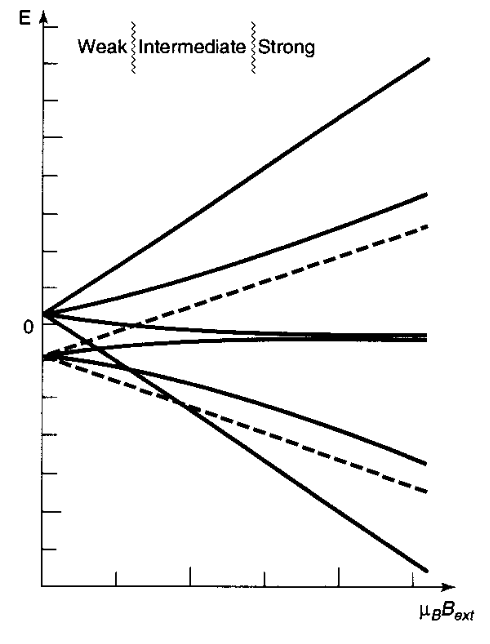
\includegraphics[width=0.6\linewidth, height=0.6\linewidth]{intermediate-split.png}
	\caption{Zeeman splitting of the $n = 2$ states of hydrogen, in the weak, intermediate and strong field regimes}
\end{figure}
\section{Hyperfine Splitting in Hydrogen}
The proton also has a magnetic dipole moment, however this is much smaller than that of the electron due to the mass of the proton. It is given by,
\begin{equation}
\mu_{p} = \frac{g_{p} e}{2 m_{p}}S_{p}
\end{equation}
And the magnetic dipole moment of the electron,
\begin{equation}
\mu_{e} = -\frac{e}{m_{e}}S_{e}
\end{equation}
Classically speaking, the dipole $\mu$ sets up a magnetic field:
\begin{equation}
B = \frac{\mu_{0}}{4 \pi r^{3}}[3(\mu . \hat{r})\hat{r} - \mu] + \frac{2 \mu_{0}}{3} \mu \delta^{3}(r)
\end{equation}
So the Hamiltonian of the electron, in the magnetic field due to the proton's magnetics dipole moment, is
\begin{equation}
H^{'}_{hf} = \frac{\mu_{0} g_{p} e^{2}}{8 \pi m_{p} m_{e}}\frac{[3(S_{p}. \hat{r})(S_{e}. \hat{r}) - S_{p}.S_{e}]}{r^{3}} + \frac{\mu_{0} g_{p} e^{2}}{3 m_{p} m_{e}}S_{p}.S_{e} \delta^{3}(r)
\end{equation}
According to perturbation theory, the first-order correcction to the energy is the expectation value of the perturbing Hamiltonian:
\begin{equation}
E^{1}_{hf} = \frac{\mu_{0} g_{p} e^{2}}{8 \pi m_{p} m_{e}} \expval{\frac{3(S_{p}.\hat{r})(S_{e}.\hat{r}) - S_{p}.S_{e}}{r^{3}}} + \frac{\mu_{0} g_{p} e^{2}}{3 m_{p} m_{e}}\expval{S_{p}.S_{e}}\abs{\psi(0)}^{2}
\end{equation}
In the groud state or any other state at which $l = 0$, the wavefunction is spherically symmetrical, and the first expectation value vanishes. Meanwhile, from the Schrodinger equation in three dimensions, we find that $\abs{\psi(0)}^{2} = 1/(\pi a^{3})$, thus,
\begin{equation}
E^{1}_{hf} = \frac{\mu_{0} g_{p} e^{2}}{3 \pi m_{p}m_{e} a^{3}}\expval{S_{p}.S_{e}}
\end{equation}
in the groud state. This is called Spin-Spin coupling because it involves the dot product of two spins in contrast with spin-orbit coupling which involves $S.L$. In the presence of spin-spin coupling, the individual spin angular momenta are no longer conserved. However the eigenvectors of the total spin is conserved:
\begin{equation}
S = S_{e} + S_{p}
\end{equation}
We square this out to get,
\begin{equation}
S_{p}. S_{e} = \frac{1}{2}(S^{2} - S^{2}_{e} - S^{2}_{p})
\end{equation}
But the electron and proton both have spin $1/2$, so $S^{2}_{e} = S^{2}_{p} = (3/4) \hbar^{2}$. In the triplet i.e. parallel spin state, the total spin is $1$, and hence $S^{2} = 2 \hbar^{2}$. In the singlet state the total spin is $0$, and  $S^{2} = 0$. Thus,
\begin{equation}
E^{1}_{hf} = \frac{4 g_{p} \hbar^{4}}{3 m_{p} m^{2}_{e}c^{2}\alpha^{4}} \begin{cases}
+1/4, & \text{ (triplet)};\\
-3/4, & \text{ (singlet)}
\end{cases}
\end{equation}
The Spin-Spin coupling breaks the spin degeneracy of the groud state, lifting the triplet and depressing the singlet, leading to an energy gap. The energy gap is given by:
\begin{equation}
\Delta E = \frac{4 g_{p} \hbar^{4}}{3 m_{p} m^{2}_{e}c^{2}\alpha^{4}} = 5.88 \times 10^{-6} \ eV
\end{equation}
\begin{figure}[h]
	\centering
	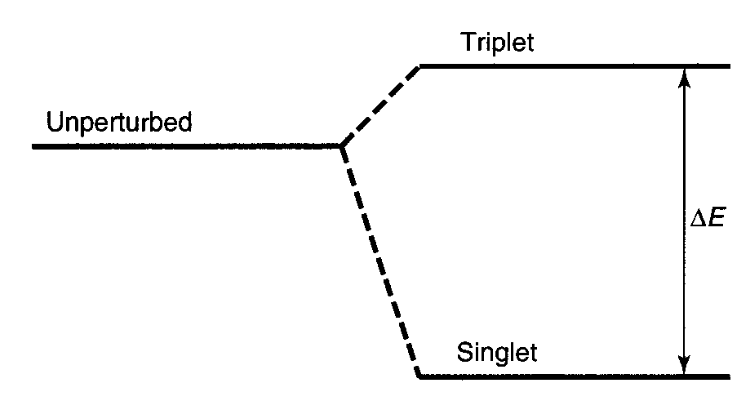
\includegraphics[width=0.6\linewidth, height=0.3\linewidth]{hyp-split.png}
	\caption{Hyperfine splitting in the ground state of Hydrogen}
\end{figure}
The frequency of the photon emitted when the triplet transitions to a singlet state is:
\begin{equation}
\nu = \frac{\Delta E}{h} = 1420 \text{ MHz}
\end{equation}
The corresponding wavelength is $21 $ cm which falls in the microwave region. It permeates the universe and is a very important part of Astrophysics.
\chapter{Scattering}
\section{Classical Scattering}
\subsection{Motivation}
We can also define the size/radius of the proton is through its rate of interacting with 	itself or other particles.
This is done by us determining the cross-sectional area. The larger this area is, the more likely it is that you will interact with it. The smaller the area, the less likely to interact.
This motivates a connection between proton size and scattering probability. In particle physics, a collision or interaction rate is expressed in effective cross-sectional area, typically just called cross section.
As an	“area,” we can measure scattering cross sections as the square of some relevant 	length scale.

\subsection{The problem}
Consider a particle incident on some scattering center. It comes in with an energy \textrm{\textit{\textbf{E}}} and an impact parameter \textrm{\textit{\textbf{b}}}, and it emerges at some scattering angle \textrm{\textit{$\theta$}}.
The essential problem of classical scattering theory is this: \textit{Given the impact parameter, calculate the scattering angle.} 
Ordinarily, of course, the smaller the impact parameter, the greater the scattering angle. 
\begin{center}
	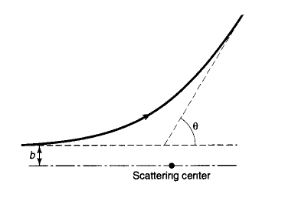
\includegraphics[scale=1.2]{ClassicalScattering}
\end{center}
\newpage

\subsection{Solving for differential cross-section}
Particles incident within an infinitesimal patch of cross-sectional area d$\sigma$ will scatter into a corresponding infinitesimal solid angle dQ. 
The larger d$\sigma$ is, the bigger dQ will be; the proportionality factor, D($\theta$) = d$\sigma$/dQ, is called the differential (scattering) cross-section, and is given by,

\begin{equation}
	d\sigma=D(\theta)d\Omega
\end{equation}
In terms of the impact parameter and the azimuthal angle $\phi, d\sigma = b.db.d\phi$ and $d\Omega=\sin(\theta)d\theta d\phi$, and so,

\begin{equation}
	D(\theta)=\frac{b}{\sin\theta}\abs{\frac{db}{d\theta}}
\end{equation}
And then the total cross-section is the integral of D($\theta$) over all solid angles,

\begin{equation}
	\sigma=\int D(\theta)d\Omega
\end{equation}

The differential cross-section is the total area of incident beam that is scattered by the target. Beams incident within this area will hit the target, and those farther out will miss it completely.\\
If we have a beam of incident particles, with uniform intensity/luminosity ($\mathcal{L}$), the number of particles entering area d$\sigma$ (and hence scattering into solid angle d$\Omega$), per unit time, is dN = $\mathcal{L}$d$\sigma$= $\mathcal{L}$D($\theta$)d$\Omega$, then,

\begin{equation}
	D(\theta)=\frac{1}{\mathcal{L}}\frac{dN}{d\Omega}
\end{equation}

This is the definition of the differential cross-section.

\begin{center}
	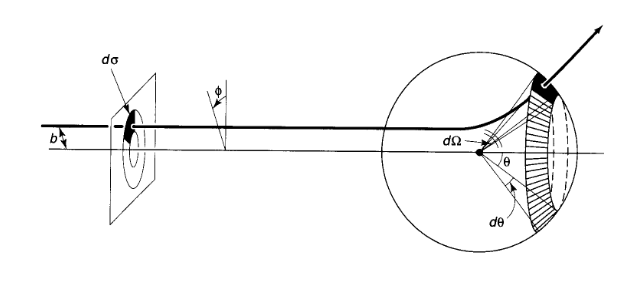
\includegraphics[scale=0.8]{DiffScattering}
\end{center}
\newpage


\section{Quantum Scattering}
\subsection{Defining the problem}
In the quantum theory of scattering, we imagine an incident plane wave,$\psi(z)=Ae^{ikz}$ , traveling in the z
direction, which encounters a scattering potential, producing an outgoing spherical wave That is, we look for solutions to the Schrödinger equation of the generic form,

\begin{equation}
	\psi(r,\theta)\approx A\left\{e^{ikz}+f(\theta)\frac{e^{ikr}}{r}\right\} \textrm{,	for large $r$}
\end{equation}

The relation between wave number $k$ and energy of incident particles are,
\begin{equation}
	k\equiv \frac{\sqrt{2mE}}{\hbar}
\end{equation}
\subsection{Determining scattering amplitude}
Probability of the incident particle travelling with speed $v$ passing through infinitesimal area $d\sigma$ in time $dt$ is,
\begin{equation}
	dP=\vert \psi_{incident}\vert^2dV=\vert A \vert^2(v dt)d\sigma
\end{equation}
This is equal to the probability that the particle later emerges into the corresponding solid angle $d\Omega$,
\begin{equation}
	dP=\vert \psi_{scattered}\vert^2dV=\frac{\vert A \vert^2\vert f \vert^2}{r^2}(v dt)r^2d\sigma
\end{equation}
And $d\sigma$=$\vert f\vert^2d\Omega$, so,
\begin{equation}
	D(\theta)=\frac{d\sigma}{d\Omega}=\vert f(\theta)\vert^2
\end{equation}
The differential cross-section (which is the quantity of interest to the experimentalist) is equal to the	absolute square of the scattering amplitude. Now we look at different methods to determine this scattering amplitude.

\newpage

\section{Partial Wave Analysis}
\subsection{Formalism}
We know that the Schrodinger equation for a spherically symmetrical potential $V(r)$ admits the separable solutions,
\begin{equation}
	\psi(r,\theta,\phi)=R(r)^m_l(\theta,\phi)
\end{equation}
Where $Y^m_l$ is a spherical harmonic and $u(R)=rR(r)$ satisfies the radial equation,
\begin{equation}
	-\frac{\hbar^2}{2m}\frac{dl^2 u}{d r^2} + \left[V(r) + \frac{\hbar^2}{2m}\frac{l(l+1)}{r^2}\right]u = Eu
\end{equation}
At very large $r$, the potential goes to zero, and the centrifugal term is negligible, so,
\begin{equation}
	\frac{d^2u}{dr^2}\approx-k^2u
\end{equation}
Whose general solution is takes the form,
\begin{equation}
	u(r)=Ce^{ikr}+De^{-ikr}
\end{equation}
The first term represents an outgoing spherical wave, and the second an incoming one. For the scattered wave, we want $D=0$. At very large r, then.
\begin{equation}
	R(r)\approx\frac{e^{ikr}}{r}
\end{equation}
The radial equation then becomes,
\begin{equation}
	\frac{d^2}{dr^2}-\frac{l(l+1)}{r^2}u=-k^2u
\end{equation}
The general solution for the radial equation is a linear combinations of spherical Bessel functions,
\begin{equation}
	u(r)=Arj_l(kr)+Brn_l(kr)
\end{equation}		
We need solutions that are linear combinations analogous to $e^ikr$ and $e^-ikr$, these are called the spherical Hankel functions,
\begin{equation}
	h^{(1)}_l\equiv j_l(x)+in_l(x)
\end{equation}
\newpage
Below we see some examples of Hankel functions,

\begin{center}
	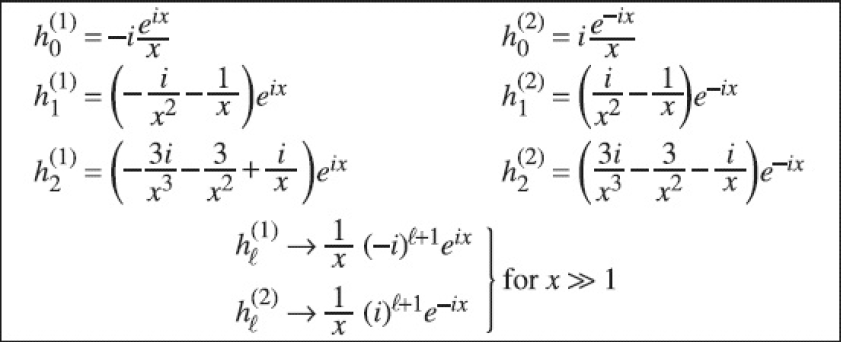
\includegraphics[scale=0.8]{Hankels}
\end{center}
The Hankel function of the first kind becomes $e^-ikr/r$ for large r, so we use these to get,
\begin{equation}
	R(r)=Cj^{(1)}_l(kr)
\end{equation}
\subsection{Exact wavefunction and the partial wave amplitude}
The exact wave function in the exterior region where $V(r)=0$ is,
\begin{equation}
	\psi(r,\theta,\phi)=A\left\{e^{ikz}+f(\theta,\phi)\frac{e^{ikr}}{r}\right\}
\end{equation}
Where,
\begin{equation}
	f(\theta,\phi)+\frac{1}{k}\sum_{l,m}^{}(-i)^{l+1}C_{l,m}Y^m_l(\theta,\phi)
\end{equation}
The $C_{l,m}$ are called the partial wave amplitudes. Now the cross section is,
\begin{equation}
	D(\theta,\phi)= \vert f(\theta,\phi)\vert^2= \frac{1}{k^2} \sum_{l,m}\sum_{l',m'}(i)^{l-l'}C^*_{l,m}C_{l'm'}(Y^m_l)^*Y^{m'}_{l'}
\end{equation}
And the total cross-section is,
\begin{equation}
	\sigma= \frac{1}{k^2} \sum_{l,m}\sum_{l',m'}(i)^{l-l'}C^*_{l,m}C_{l'm'}\int(Y^m_l)^*Y^{m'}_{l'}d\Omega=\frac{1}{k^2}\sum_{l,m}^{}\vert C_{l,m}\vert ^2
\end{equation}
We know from the Legendre functions that,
\begin{equation}
	Y^0_l(\theta,\phi)=\sqrt{\frac{2l+1}{4\pi}}P_l(cos\theta)
\end{equation}
where $P_l$ is the $l$th Legendre Polynomial. Now the exact wave function in the exterior region is,
\begin{equation}
	\psi(r,\theta)=A\left\{e^{ikz}+\sum_{l=0}^{\infty}\sqrt{\frac{2l+1}{4\pi}}C_lh_l^{(1)}(kr)P_l(cos\theta)\right\}
\end{equation}
The scattering amplitude is now given by,
\begin{equation}
	f(\theta)=\frac{1}{k}\sum_{l=0}^{\infty}(-i)^{l+1}\sqrt{\frac{2l+1}{4\pi}}C_lP_l(cos\theta)
\end{equation}
and the total cross-section is,

\begin{equation}
	\sigma=\frac{1}{k^2}\sum_{l=0}^{\infty}|C_l|^2
\end{equation}
To fix the hybrid notation of the cartesian incoming wave and the spherical outgoing wave, we write it in a more consistent form.\\ 
We know that the general solution to the Schrodinger equation with $V=0$ can be written in the form,
\begin{equation}
	\sum_{l,m}^{}[A_{l,m}j_l(kr)+B_{l,m}n_l(kr)]Y^m_l(\theta,\phi)
\end{equation}
Expanding the plane wave in terms of spherical waves using Rayleigh's formula,
\begin{equation}
	e^{ikz}=\sum_{l=0}^{\infty}i^l(2l+l)j_l(kr)P_l(cos\theta)
\end{equation}
Substituting this in Equation (24), the consistent exterior region wave function can be written as,
\begin{equation}
	\psi(r,\theta)=A\left[l(2l+l)j_l(kr)+\sum_{l=0}^{\infty}\sqrt{\frac{2l+1}{4\pi}}C_lh_l^{(1)}(kr)\right]P_l(cos\theta)
\end{equation}

\section{Phase Shift}
Let's begin by considering a one-dimensional scattering problem with a localized potential on the half-line $x < 0$ and a brick wall at $x = 0$. So a wave incident from the left,
\begin{equation}
\psi_{i}(x) = A e^{ikx}
\end{equation}
is entirely reflected,
\begin{equation}
\psi_{r}(x) = B e^{-ikx}
\end{equation}
\begin{figure}[h]
	\centering
	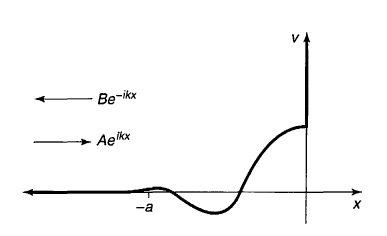
\includegraphics[scale=0.6]{1d_scatt.png}
	\caption{1D scatterubg frin a localized potential bounded on the right by an infinite wall}
\end{figure}
where $x < -a$. No matter what happens in $-a < x < 0$ (the interaction region), the amplitude (amplitude in the context of waves not probability amplitude) of the reflected wave is the same as the incident wave simply due to conservation of probability. However, the two waves need not have the same phase. If there were no potential at all ($V(x) = 0$), but just at the wall ($x = 0$), then $B = -A$, since the total wave function, incident + reflected must vanish at the origin,
\begin{equation}
\psi_{0} = A (e^{ikx} - e^{-ikx})
\end{equation}
If the potential is not zero ($V(x) \neq 0$), then the wave function ($x < -a$) takes the form:
\begin{equation}
\psi = A \left(e^{ikx} - e^{i(2 \delta - kx)} \right)
\end{equation}
Thus, the whole scattering problem reduces to the problem of calculating the phase shift $\delta$ as a function of $k$ and hence of the Energy $E = \hbar^{2}k^{2}/2m$. Yes there's a factor of 2, before $\delta$, but that's only conventional. We think of the incident wave as being phase shifted once on the way in and again on the way out. Thus, by $\delta$ we mean the one-way phase shift and $2\delta$ the total phase shift. We go about this by solving the Schrodinger equation in $-a < x < 0$ along with relevant boundary conditions. Why are we working with $\delta$ rather than the complex amplitude $B$? It makes the physics and math simpler:
\begin{itemize}
\item \textbf{Physically:} We only need to think of the conservation of probability. The potential merely shifts the phase
\item \textbf{Mathematically:} We trade a complex number for a real one
\end{itemize}
Let's return to the 3D  case. The incident plane wave carries no angular momentum in the z direction. Thus Rayleigh's formula contains no terms with $m \neq 0$ but insteaed it cfontains all values of the total angular momentum ($l = 0, 1, 2$). Since angular momentum is conserved by a spherically symmetric potential each partial wave labelled by a particular $l$ scatters independently with no change in amplitude (amplitude in this context refer to the amplitude of the wave no the probability amplitude) but differing in phase. If there is no potential then $\psi_{0} = A e^{ikx}$ and the $l$th partial wave is
\begin{equation}
\psi^{l}_{0} = A i^{l} (2l +1) j_{l}(kr)P_{l}(\cos(\theta))
\end{equation}
But from our previous considerations,
\begin{equation}
j_{l}(x) = \frac{1}{2} \left[h^{(1)}(x) + h^{2}_{l}(x) \right] \approx \frac{1}{2x} \left[(-i)^{l+1} e^{ix} + i^{l+1}e^{-ix} \right]
\end{equation}
for $x >>1$. So for large $r$,
\begin{equation}
\psi^{(l)}_{0} \approx A \frac{2l + 1}{2ikr} \left[e^{ikr} - {(-1)}^{l}e^{-ikr}\right] P_{l}(\cos(\theta))
\end{equation}
The second term in square brackets corresponds to an incoming spherical wave. It is unchanged when we introduce the scattering potential. The first term is the outgoing wave. It picks up a phase shift $\delta_{l}$:
\begin{equation}
	\label{tobeass}
\psi^{(l)} \approx A \frac{2l + 1}{2ikr} \left[e^{i(kr + 2\delta_{l})} - {(-1)}^{l}e^{-ikr}\right] P_{l}(\cos(\theta))
\end{equation}
Think of it as a converging spherical wave due to the $h^{(2)}_{l}$ component in $e^{ikz}$, which is phase shifted by $2\delta_{l}$ and emerges as an outgoing spherical wave i.e. the $h^{l}_{l}$ part of $e^{ikz}$ as well  as the scattered wave itself. In the previous section the whole theoryu was expressed in terms of partial wave amplitudes $a_{l}$, now we have formulated it in terms of the phase shifts $\delta_{l}$. There must be a connectioni between the two. Well if we take the assymptotic i.e. large $r$ limit of eq. (\ref{tobeass}):
\begin{equation}
\psi^{(l)} \approx A\left( \frac{(2l + 1)}{2ikr} \left[e^{i(kr + 2\delta_{l})} - {(-1)}^{l}e^{-ikr}\right] + \frac{(2l + 1)}{r}a_{l}e^{ikr} \right) P_{l}(\cos(\theta))
\end{equation}
With the generic expression in terms of $e^{i \delta_{l}}$ we find
\begin{equation}
a_{} = \frac{1}{2ik}(e^{2i \delta_{l}} - 1) = \frac{1}{k} e^{i \delta_{l}} \sin(\delta_{l})
\end{equation}
Although we used the assymptotic form of the wave function to find the connection there's nothing approximate about the result. Both of them are constants independent of $r$ and $\delta_{l}$ means the phase shift in the asymptotic region i.e. where the Hankel functionis have settled down to $e^{\pm ikr}/kr$. It follows in particular that,
\begin{equation}
f(\theta) = \frac{1}{k}\sum_{l=0}^{\infty}(2l + 1)e^{i \delta_{l}} \sin(\delta_{l}) P_{l}(\cos(\theta)) 
\end{equation}
and,
\begin{equation}
\sigma = \frac{4 \pi}{k^{2}} \sum_{l=0}^{\infty}(2l + 1) \sin[2](\delta_{l})
\end{equation}
Voila!
\section{Born Approximation}
\subsection{Integral Form of the Schrodinger Equation}
Before we even head to deriving the "Integral Form of the Schrodinger Equation". Why you might ask? It will become evident in the upcoming sections. So let's begin by recalling the time-independent Schrodinger equation
\begin{equation}
\frac{num}{2m} + V \psi = E \psi
\end{equation}
We can rewrite this as,
\begin{equation}
(\nabla^{2} + k^{2}) \psi = Q
\end{equation}
where
$$k = \frac{\sqrt{2mE}}{\hbar}$$
$$Q = \frac{2m}{\hbar^{2}}V \psi$$
This looks pretty similar to the Helmholtz equation from electrodynamics. Here however the "inhomogeneous" term Q itself depends on $\psi$
Suppoase we could find a function that solves the Helmholtz equation with a delta function source:
\begin{equation}
(\nabla^{2} + k^{2}) G(\vec{r}) = \delta^{3}(\vec{r})
\end{equation}
We can then express as an integral:
\begin{equation}
	\psi(\vec{r}) = \int G(\vec{r} - \vec{r_{0}}) Q(\vec{r_{0}}) d^{3}\vec{r_{0}}
\end{equation}
$G(\vec{r})$ is called the Green's function for the Helmholtz equation. Moreover, generally speaking the Green's function for a linear differential equation represents the response to a delta function. Our goal now is to solve this differential equation, we start by Fourier transforming it to turn it into an algebraic equation:
\begin{equation}
G(\vec{r}) = \frac{1}{{(2 \pi )}^{3/2}} \int e^{i \vec{s}. \vec{r}} g(\vec{s}) d^{3}\vec{s}
\end{equation}
Then,
$$(\nabla^{2} + k^{2}) G(\vec{r}) = \frac{1}{{(2 \pi)}^{3/2}} (\nabla^{2} + k^{2})\int e^{i \vec{s}. \vec{r}} g(\vec{s}) d^{3}\vec{s}$$
But,
$$\nabla^{2}e^{i \vec{s}. \vec{r}} = -s^{2}e^{i \vec{s}. \vec{r}}$$
and
$$\delta^{3}(\vec{r}) = \frac{1}{{(2 \pi )}^{3/2}} \int e^{i \vec{s}. \vec{r}} g(\vec{s}) d^{3}\vec{s}$$
thus,
$$\frac{1}{den} = \frac{1}{den} \int e^{i \vec{s}. \vec{r}} d^{3}\vec{s}$$
It follows from Plancherel's theorem that,
$$g(\vec{s}) = \frac{1}{{(2 \pi)}^{3/2}(k^{2} - 2^{2})}$$
Plugging this back, we see that
$$G(\vec{r}) = \frac{1}{{(2 \pi)}^{3}}  \int e^{i \vec{s}. \vec{r}} \frac{1}{(k^{2} - 2^{2})} d^{3}\vec{s}$$
We now switch coordinates for convenience. Now $\vec{r}$ is fixed as far as the $s$ integration matters so we'll choose spherical coordinates with the polar axis along $\vec{r}$. Then 
$$\int^{2 \pi}_{0} e^{isr \sin(\theta)} \sin(\theta) d \theta = - \frac{e^{isr \cos(\theta)}}{isr} \Big \rvert^{\pi}_{0} = \frac{2 \sin(sr)}{sr}$$
We can represent this visually as,
\begin{figure}[h]
	\centering
	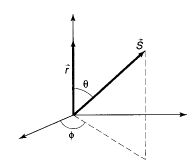
\includegraphics[scale=0.6]{scatter_coord.png}
	\caption{New coordinates for the integral}
\end{figure}
Thus,
$$G(\vec{r}) =  \frac{1}{{(2 \pi)}^{2}}\frac{2}{r} \int^{\infty}_{0} \frac{s \sin(sr)}{k^{2} - s^{2}} ds = \frac{1}{4 \pi^{2} r}\int^{\infty}_{-\infty} \frac{s \sin(sr)}{k^{2} - s^{2}} ds$$
We can rewrite this as,
$$G(\vec{r}) = \frac{i}{8 \pi^{2} r} \left[\int_{-\infty}^{\infty} \frac{se^{isr}}{(s-k)(s+k)} ds - \int_{-\infty}^{\infty} \frac{se^{-isr}}{(s-k)(s+k)} ds \right] = \frac{i}{8 \pi^{2} r}(I_{1}-I_{2})$$
From Cauchy's integral formula it follows that,
$$I_{1} = \oint \left[\frac{se^{isr}}{s + k} \right] \frac{1}{s-k}ds = 2 \pi i \left[ \frac{s e^{isr}}{s + k} \right] \Big \rvert_{{s= k}}  = i \pi e^{ikr}$$
$$I_{2} = \oint \left[\frac{se^{-isr}}{s - k} \right] \frac{1}{s+k}ds = -2 \pi i \left[ \frac{s e^{isr}}{s + k} \right] \Big \rvert_{{s= -k}}  = -i \pi e^{ikr}$$
%\big{\vert_{s = -k}}
Therfore,
\begin{equation} \label{b1}
G(\vec{r}) = \frac{i}{8 \pi^{2} r} \left[ \left(i \pi e^{ikr} \right) - \left(-i \pi e^{ikr} \right) \right] = -\frac{e^{ikr}}{4 \pi r}
\end{equation}
Note that $G + G_{0}$ still satisfies Equation (\ref{b1}). This is simply due to the multivalued nature of the holomorphic function. Thus, the integral form of the Schrodinger equation can be written as,
\begin{tcolorbox}
\begin{equation}
\psi(\vec{r}) = \psi_{0}(\vec{r}) - \frac{m}{2 \pi \hbar^{2}}\int\frac{e^{ik\abs{\vec{r} - \vec{r}_{0}}}}{\abs{\vec{r} - \vec{r}_{0}}}  V(\vec{r}_{0}) \psi(\vec{r}_{0}) d^{3}\vec{r}_{0}
\end{equation}
\end{tcolorbox}
Let's see how this helps us.
\subsection{The First Born Approximation}
Suppose $V(\vec{r}_{0})$ is localized about r = 0, that is the potential drops to 0 after a finite region and we want to calculate $\psi(\vec{r})$ at points distant from the scattering center. Then for all points that contribute to the integral form of the Schrodinger equation. So,
\begin{equation}
\abs{\vec{r} - \vec{r}_{0}} = r^{2} + r_{0}^{2} - 2\vec{r}\vec{r_{0}}  \approxeq r^{2} \left(1 - 2\frac{\vec{r}.\vec{r}_{0}}{r^{2}} \right)
\end{equation}
and hence,
\begin{equation}
\abs{\vec{r} - \vec{r}_{0}} \approxeq r - \hat{r} . \vec{r}_{0}
\end{equation}
Let,
\begin{equation}
\vec{K} = k \hat{z}
\end{equation}
then
\begin{equation}
e^{-i \vec{K}\abs{\vec{r} - \vec{r}_{0}}} \approx e^{ikr}e^{-i \vec{K}.\vec{r}_{0}}
\end{equation}
and therefore,
\begin{equation}
\frac{e^{-i \vec{K}\abs{\vec{r} - \vec{r}_{0}}}}{\abs{\vec{r} - \vec{r}_{0}}} \approx \frac{e^{ikr}}{r}e^{-i \vec{K}.\vec{r}_{0}}
\end{equation}
In the case of scattering, we want:
\begin{equation}
\psi_{o}(\vec{r}) = Ae^{ikz}
\end{equation} 
to represent an incident plane wave. For large $r$,
\begin{equation}
\psi \approxeq Ae^{ikz} - \frac{m}{2 \pi \hbar^{2}A} \int e^{-i \vec{K}.\vec{r}_{0}}V(\vec{r}_{0})\psi(\vec{r}_{0})d^{3}\vec{r}_{0}
\end{equation}
This is in the standard form. We can read off the scattering amplitude:
\begin{equation}
f(\theta, \phi) = \frac{m}{2 \pi \hbar^{2}A} \int e^{-i \vec{K}.\vec{r}_{0}}V(\vec{r}_{0})\psi(\vec{r}_{0})d^{3}\vec{r}_{0}
\end{equation}
So far this is exact. Now we invoke the Born approximation: "Suppose the incoming plane wave is not substantially altered by the potential; then we can say that
\begin{equation}
\psi(\vec{r}_{0}) \approxeq \psi_{0}(\vec{r}_{0}) = A e^{ikz_{o}} = A e^{i\vec{K}^{'}\vec{r}_{o}}
\end{equation}
where
$$K^{'}= k \hat{z}$$
inside the integral. This would be just the wave function if $V$ were zero. It is essentially just a weak potential approximation. Generally partial wave analysis is useful when the incident particle has low energy the only the first few terms in the series contribute significantly. The Born approximation applies when the potential is weak when compared to the incident energy, thus the deflection is small. In the Born approximation then,
\begin{tcolorbox}
	\begin{equation}
		f(\theta, \phi) \approxeq -\frac{m}{2 \pi \hbar^{2}} \int e^{i(k^{'}-k). \vec{r}_{0}}V({r}_{0})d^{3}\vec{r}_{0}
	\end{equation}
\end{tcolorbox}
In particular, for low energy scattering, the exponential factor is essentially constant over the scattering region and the Born approximation simplifies to:
\begin{tcolorbox}
	\begin{equation}
		f(\theta, \phi) \approxeq -\frac{m}{2 \pi \hbar^{2}} \int V(\vec{r}) d^{3}r
	\end{equation}
\end{tcolorbox}
For a spherically symmetrical potential, $V(\vec{r}) = V(r)$ but not necessarily at low energy. The Born approximation reduces to a simpler form. First we define:
\begin{equation}
\mathcal{K} = k^{'} - k
\end{equation}
and let the polar axis for the $r_{0}$, the integral lies along so that;
\begin{equation}
(k^{'} - k).r_{0} = \mathcal{K}r_{0} \cos(\theta_{0})
\end{equation}
Then,
\begin{equation}
f(\theta) \approxeq -\frac{m}{2 \pi \hbar^{2}} \int e^{i \mathcal{K} r_{0} \cos(\theta_{0})} V(\theta_{0}) r^{2}_{0} \sin(\theta_{0}) dr_{0}d \theta_{0} d \phi_{0}
\end{equation}
The integral is trivial, $2\pi$, and the integral $\theta_{0}$ is on we have encountered before in equation (). Dropping the subscript on $r$, we are left with
\begin{tcolorbox}
\begin{equation}
f(\theta) \approxeq -\frac{2m}{\hbar^{2} \mathcal{K}} \int_{0}^{\infty} rV(r)\sin(\mathcal{K}r) dr
\end{equation}
\end{tcolorbox}
The angular dependence of $f$ is carried by $\mathcal{K}$. From our previous considerations we can see that:
\begin{equation}
\mathcal{K} = 2k \sin(\theta /2)
\end{equation}
\subsection{Examples}
\subsubsection{Low-energy soft-sphere scattering}
Note: We can't apply the Born approximationi to hard-sphere scattering as the integral blows up due to our assumption (i.e. potential does not affect the wave function) here. Suppose,
\begin{equation}
	V(\vec{r}) = \begin{cases}
		V_{0}, & \text{ if } r \leq a \\
		0, & \text{ if } r > a
	\end{cases}
\end{equation}
In this case the low-energy scattering amplitude is,
\begin{equation}
	f(\theta, \phi) \approxeq -\frac{m}{2 \pi \hbar^{2}}V_{0}\left(\frac{4}{3} \pi a^{3} \right)
\end{equation}
This is independent of $\theta$ and $\phi$ ! Thus, the differential cross-section is:
\begin{equation}
\frac{d \sigma}{d \Omega} = \abs{f}^{2}  \approxeq \left[\frac{2m V_{0} a^{3}}{3 \hbar^{2}} \right]^{2}
\end{equation}
and the total cross-section:
\begin{equation}
\sigma 	\approxeq 4 \pi \left(\frac{2m V_{0} a^{3}}{3 \hbar^{2}}\right)^{2}
\end{equation}
\subsubsection{Yukawa Scattering}
The Yukawa potential is a toy-model for the binding force in the nucleus of an atom. It has the form,
\begin{equation}
V(r) = \beta \frac{e^{-\mu r}}{r}
\end{equation}
where $\beta$ and $\mu$ are constants. The Born approximation gives,
\begin{equation}
f(\theta) \approxeq -\frac{2m \beta}{\hbar^{2}k} \int_{0}^{\infty} e^{- \mu r} \sin(kr) dr = - \frac{2m \beta}{\hbar^{2} (\mu^{2} + k^{2})}
\end{equation}
\subsubsection{Rutherford Scattering}
If we substitute $\beta = q_{1}q_{2}/ 4 \pi \epsilon_{0}$ and $\mu = 0$. The scattering amplitude is given by,
\begin{equation}
f(\theta) \approxeq - \frac{2m q_{1}q_{2}}{4 \pi \epsilon_{0} \hbar^{2} k^{2}}
\end{equation}
or,
\begin{equation}
f(\theta) \approxeq - \frac{q_{1}q_{2}}{16 \pi \epsilon_{0} E \sin[2](\theta / 2)}
\end{equation}
The differential cross-section is the square of this:
\begin{equation}
	\frac{d \sigma}{d \Omega} = \left[\frac{q_{1}q_{2}}{16 \pi \epsilon_{0} E \sin[2](\theta / 2)} \right]^{2}
\end{equation}
\subsection{The Born series}
The Born approximation is very similar to the impulse approximation in the contex of classical scattering. 
\begin{figure}[h]
	\centering
	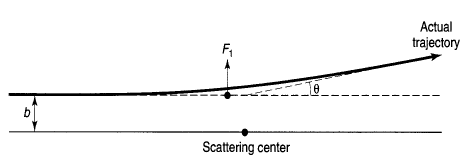
\includegraphics[scale=0.5]{impulse_scatt.png}
	\caption{An example of the impulse approximation: the particle continues undeflected}
\end{figure}
In that sector we start by assuming that the particle keeps going in a straight line and compute the transverse impulse that would be delivered to it in that case:
\begin{equation}
I = \int F_{\perp} dt
\end{equation}
If the deflection is small in comparism to the motion, it would then be a good approximation to the transverse momentum supplied to th particle. Thus we express the scattering angle as:
\begin{equation}
\theta = \arctan(I/p)
\end{equation}
where $p$ is th incident momentum. This is the "first-order" impulse approximation. The zeroth-order is what we started wtih i.e. no deflection at all. Likewise, in the zeroth-order Born approximation the incident plane wave passes by with no modification and what we saw earlier was just the first order correction to this. But the same pattern of thought can lead us to a series which then leads us to higher-order corrections. Let's recall the integral form of the Schrodinger equation:
\begin{equation}
		\label{schrod_int_2}
	\psi (\vec{r}) = \psi_{0} (\vec{r}) + \int g(\vec{r} - \vec{r}_{0})V(\vec{r}_{0})\psi(\vec{r}_{0})d^{3}r_{0}
\end{equation}
where is the incident wave and,
$$g(\vec{r}) = -\frac{m}{2 \pi \hbar^{2}}\frac{e^{ikr}}{r}$$
is the Green's function with a factor $m/2 \pi \hbar^{2}$ for convenience and $V$ is the scattering potential.
Suppose we take the equation for $\psi$ and plug it back into (\ref{schrod_int_2}),
$$\psi = \psi_{0} + \int g V\psi_{0} + \int \int g V g V\psi$$
Iterating this we obtain the series expasion for $\psi$,
\begin{equation} 
	\label{dysonseries}
\psi = \psi_{0} + \int g V\psi_{0} + \int \int g V g V\psi_{0} + \int \int \int g V g V g V\psi_{0} ...
\end{equation}
\begin{figure}[h]
	\label{born_diag}
	\centering
	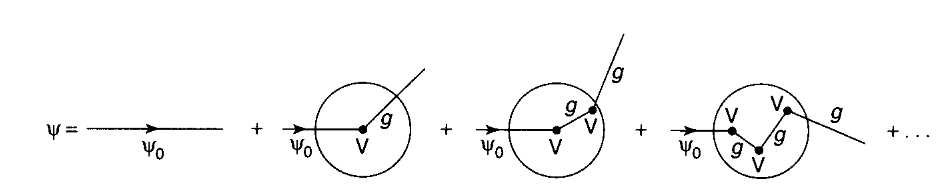
\includegraphics[scale=0.5]{born_series.png}
	\caption{A diagram representing the Born series}
\end{figure}
We notice the following from (\ref{dysonseries}):
\begin{itemize}
\item The first Born approximation truncates the series after the Next to Leading Order (NLO) term
\item In the Leading Order $\psi$ is untouched by $V$
\item In the first order (Next to Leading Order) it is kicked once
\item In the second order it is kicked, propagates to a new location and is kicked again and so on
\item In this context the Green's function is essentially just the propagator \footnote{In this context it tells us how the disturbance propagates between one interaction and the next}
\item This was in fact the inspiration for Feynman diagrams which is expressed in terms of vertex factors ($V$) and propagators ($g$)
\end{itemize}
Figure (\ref{born_diag}) might look familiar, because it closely represents Feynman diagrams.
\begin{figure}[h]
	\centering
	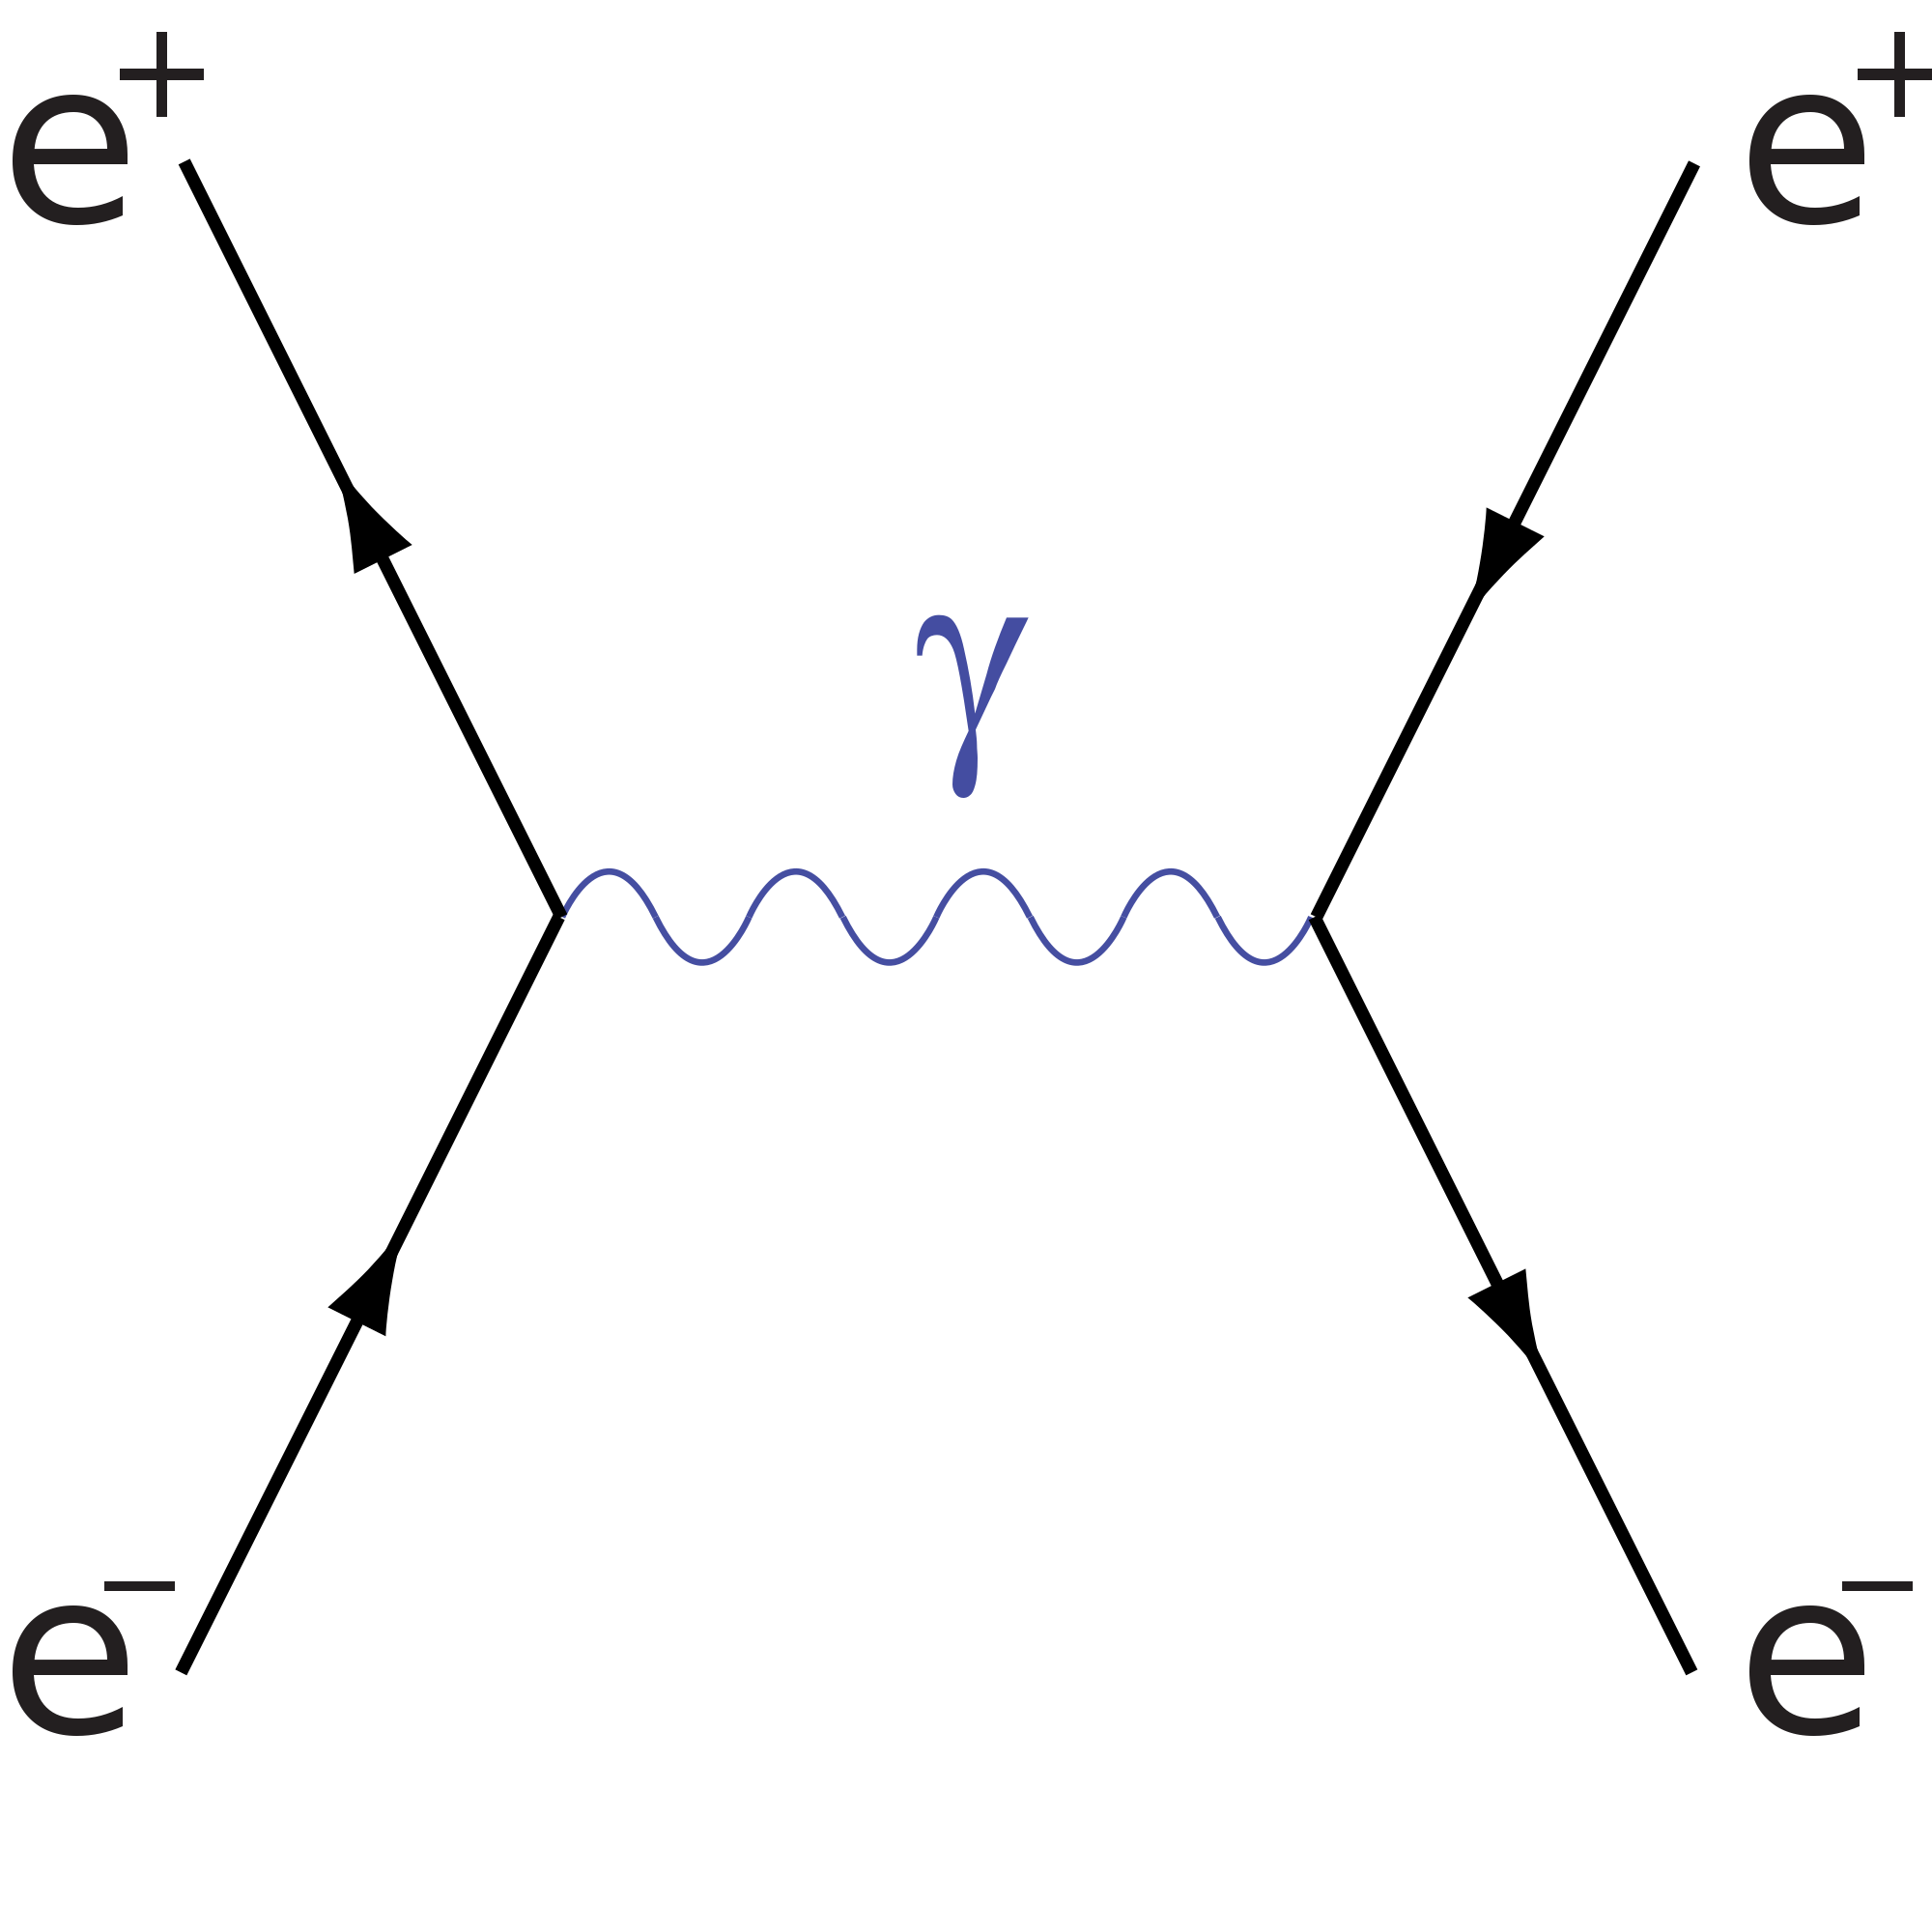
\includegraphics[scale=0.1]{2000px-Bhabha_S_channel.svg}
	\caption{Bhabha scattering: Annihilation}
\end{figure}
\chapter{Graphs \& Combinotorial Optimization}
\section{Combinotorial Optimization} 
Combinotorial Optimization concerns optimization problems of a discrete or combinatorial strcuture. It uses graphs and digraphs as basic tools.
\section{Graphs}

\section{Digraphs}
\section{Shortest Path Problems}
\subsection{Complexities}
\section{Bellman's Principle}
\section{Dijkstra's Algorithm}
\section{Shortest Spanning Trees}
\subsection{Greedy's Algorithm}
\subsection{Prim's Algorithm}
\section{Flows in Networks}
\subsection{Maximum Flow: Ford-Fulkerson Algorithm}
\section{Bipartite Graphs}

\chapter{Relativistic Quantum Mechanics}
\section{The Klein-Gordon Equation}
In order to develop quantum mechanics relativistically, they started from the relativistic
energy–momentum relation,
\begin{equation}
	E^2 - \big|\vec{p}\big|^2c^2 -m^2c^4 = 0
\end{equation}
Substituting $E$ and $p$ for their respective operators,

$$E \Rightarrow i\hbar\frac{\partial }{\partial t},\hspace{50pt}\vec{p} \Rightarrow -i\hbar\vec{\nabla},$$ 

and letting the equation act on a wavefunction $\phi(\vec{x} , t)$  the equation becomes,
\begin{equation}
	\Big( -\hbar^2\frac{\partial^2 }{\partial t^2} + \hbar^2c^2\nabla^2 - m^2c^4 \Big)\phi(\vec{x} , t) = 0
\end{equation}

This is the Klein-Gordon Equation. The wave function $\phi(\vec{x} , t)$ is also an object called a field because its arguments extend over all space and time. Another way to say this is that it exists
throughout spacetime and its fluctuations are described by the Klein–Gordon
equation. In natural units,
$$\Big( \frac{\partial^2}{\partial t^2} + \nabla^2 - m^2 \Big)\phi(\vec{x},t) = 0$$

This equation was the first attempt at a relativistic quantum mehcanical equation of a wave. it tells us how the field of a particle fluctuates.

The Klein-Gordon equation can also be written in the Lorentz-invariant form,
\begin{equation}
	(\partial^\mu\partial_\mu+m^2)\psi=0
\end{equation}

Where,
\begin{equation*}
	\partial^\mu\partial_mu\equiv\frac{\partial^2}{\partial t^2}- \frac{\partial^2}{\partial x^2}-\frac{\partial^2}{\partial y^2}-\frac{\partial^2}{\partial z^2}
\end{equation*}
The Klein-Gordon equation has plane wave solutions,
\begin{equation}
	\psi(x,t)=Ne^{i(p\cdot x-Et)}
\end{equation}

Substituting in Equation (3),
\begin{equation*}
	E^2\psi=p^2\psi+m^2\psi
\end{equation*}
\section{The Dirac Equation}
\section{Covariant Formalism}
\subsection{The Adjoint Spinor and the Covariant Current}
\section{Solutions to the Dirac Equation}
\subsection{Particles at Rest}
\subsection{General Free-Particle Solutions}
\section{Antiparticles}
\subsection{The Dirac Sea Interpretation}
\subsection{The Feynman-Stuckelberg Interpretation}
\subsection{Antiparticle Spinors}
\chapter{Statistics}

\chapter{A Historical Overview}
Rishi's article + JP sir's slides
\section{Blackbody Radiation}
\section{Premise}
We can consider a black body to consist of electromagnetic radiation in thermal equilibrium with the walls of the cavity. When they are in thermal equilibrium, the average rate of emission of radiation equals their average rate of absorption of radiation. \\

\noindent The Rayleigh Jeans theory was constructed on the notion that when the walls of an object is in thermal equilibrium, in other words, the temperature of the walls is equal to the "temperature" of radiation. We will see what we mean by the "temperature" of an electromagnetic wave. \\

\noindent If we take the walls of a cavity to consist of oscillating charged particles (about its equilibrium) coupled to a standing-wave mode of an electromagnetic field. This can be seen from Maxwell's theory of electromagnetic waves, which states that a moving charged particle radiates an electromagnetic wave. A point to be noted is that the frequency of the oscillating charge is equal to the frequency of its coupled electromagnetic wave. So then, it is safe to say that in thermal equilibrium, the average energy of the oscillating charge is equal to the average energy of the coupled standing-wave mode of that electromagnetic field. \\

\noindent Now we can see that the oscillating particle has a quadratic potential energy, $H_{pot}$  of $\frac{1}{2}aq^2$ and a kinetic energy $H_{kin}$ of $\frac{p^2}{2m}$, so according to the equipartition theorem, in thermal equilibrium the average energy is,
\begin{equation}
	\braket{H}=\braket{H_{pot}}+\braket{H_{kin}}=\frac{1}{2}k_BT+\frac{1}{2}k_BT=k_BT
\end{equation}	
Hence the energy of the wave is also taken to be $k_BT$, and can be thought to have a "temperature" of T. \\

\noindent This forms the foundation of the Rayleigh Jeans theory, following which we will derive the Rayleigh-Jeans formula.

\newpage
\section{Deriving the Rayleigh-Jeans Formula}
We start off with the axiom that the energy distribution of a black-body radiation does not depend on the shape of the cavity (which can be proven experimentally). For ease of calculations, we take te shape of the cavity to be a cube. We also assume that the waves vanish at the walls, or in other words, do not pass through them.\\
\noindent The number of standing electromagnetic waves in a cube of length L needs to be calculated. \\
Let us take the wave equation for the standing electromagnetic wave,
\begin{equation}
	\frac{\partial^2E_x}{\partial x^2}+\frac{\partial^2E_x}{\partial y^2}+\frac{\partial^2E_x}{\partial z^2}+k^2E_x=0
\end{equation}
Where $E_x=E_x(x,y,z)$ and $k=\frac{2\pi}{\lambda}=\frac{2\pi f}{c}$.
Assuming that $E_x=u(x)v(y)w(z)$ (by variable separable method), we can separate Equation (2) into three ordinary differential equations of the type,
\begin{equation}
	\frac{d^2u}{dx^2}+k^2_xu=0
\end{equation}
Where $k^2=k^2_x+k^2_y+k^2_z$. By inspection, we can see that Equation (3) is an equation for a simple harmonic oscillator and has the solution,
\begin{equation}
	u(x)=B\cos k_xx+C\sin k_xx
\end{equation}
Applying necessary boundary conditions so that $E_x$ or $u$ is 0 at $x=0$ and at $x=L$ leads to $B=0$ and $k_xL=n_x\pi$ where $n_x=1,2,3,...$, (since we are considering standing electromagnetic waves and look at only the positive region of the k-space) similar solutions are obtained for $v(y)$ and $w(z)$, giving the solution,
\begin{equation}
	E_x(x,y,z)=A\sin (k_xx)sin(k_yy)\sin(k_zz)
\end{equation}
Where,
\begin{equation}
	k^2=\frac{\pi ^2}{L^2}(n^2_x+n^2_y+n^2_z)
\end{equation}
and $n_x$, $n_y$ and $n_z$ are postive integers.\\
Now, we take Equation (6) to give us the distance from the origin to a point in $k$-space, or often called the "Reciprocal" space (due to the units of $k$ being $(length)^-1$).\\
Let us take a coordinate system corresponding to the $k$-space (as shown in Figure 1), with the axes being $k_x$, $k_y$ and $k_z$. And we know that $k_x=n_x\pi/l$, $k_y=n_y\pi/L$, and $k_z=n_z\pi/L$, so the points in $k$-space are separated by $\pi/L$ along each axis, and there is one standing wave in $k$-space per $(\pi/L)^3$ of volume. The number of standing waves, $N(k)$ having wavenumbers between $k$ and $k+dk$ is then simply the volume between $k$ and $k+dk$ divided by $(\pi/L)^3$. The volume between $k$ and $k+dk$ is simply the volume of a spherical shell of thickness $dk$ multiplied by $1/8$ (since we need only the positive quadrant of the k-space, hence 1/4 of the volume of sphere), so that
\begin{equation}
	N(k)dk=\frac{\frac{1}{2}\pi k^2dk}{(\pi/L)^3}=\frac{Vk^2dk}{2\pi^2}
\end{equation}
Where $V=L^3$ is the volume of the cavity.\\
For any electromagnetic wave, there are two perpendicular polarisations for each mode, so Equation (6) should be increased by a factor of 2, becoming,
\begin{equation}
	\frac{N(k)dk}{V}=\frac{k^2dk}{\pi^2}
\end{equation}
From using the expression $k=2\pi f/c$ to obtain $k$ and $dk$ and substituting in Equation (8) gives us $N(f)$,
\begin{equation}
	N(f)df=\frac{8\pi f^2}{c^3}df
\end{equation}
And from this, the number of modes per unit volume between $\lambda$ and $\lambda + d\lambda$ can be derived from Equation (9) by using the expression $f=c/\lambda$ to get $\lambda$ and $d\lambda$ to get,
\begin{equation}
	N(\lambda)d\lambda=\frac{8\pi}{\lambda^4}d\lambda
\end{equation}
Now, each mode of oscilation has energy of $k_BT$, so the energy in the range $\lambda$ to $\lambda+d\lambda$ is $k_BTN(\lambda)d\lambda$. Hence the energy density in this region is,
\begin{equation}
	u(\lambda)d\lambda = k_BTN(\lambda)=\frac{8\pi k_BT}{\lambda^4}d\lambda
\end{equation}
This is the Rayleigh Jeans expression for spectral density in the range $\lambda$ to $d\lambda$
Considering the energy to be a continuous variable, then the average energy per oscillator is $k_BT$ and the Rayleigh Jeans formula for $u(\lambda)$ holds true. The Rayleigh Jeans formula also behaves perfectly well for long wavelengths in the electromagnetic spectum. It also agrees with the Wien's scaling formula,
\begin{equation}
	u(\lambda)=\frac{8\pi k_BT}{\lambda^4}=\frac{f(\lambda T)}{\lambda^5}
\end{equation}
However, we will see in the next section why this is not a correct scaling function.\\
\begin{figure}[h]
	\centering
	\includegraphics[width=0.7\linewidth]{"Oscillation modes"}
	\caption[Visualising the k-space]{Visualising the k-space}
	\label{fig:oscillation-modes}
\end{figure}
\newpage
\section{Failure of the Rayleigh Jeans theory in explaining the Stefan-Boltzmann Law}
\subsection{Incorrect Scaling function}
From the previous equation for the scaling function, we can see that $f(\lambda T)=8k_BT$. So from this, we can notice that as $\lambda$ decreases, the u($\lambda$) also increases. This means that higher the temperature, more lower wavelength waves are emitted, for example, a campfire emits a large amount of short wavelength microwaves (which is very deadly, but thankfully that isnt how things work in nature) according to this law. Hence, the law fails in this regard.

\subsection{The Ultraviolet Catastrophe}
Inspecting the Rayleigh-Jeans formula, and attempting to find the total energy density (by integrating with appropriate limits) of the black body gives us an interesting result,
\begin{equation}
	u=\int_{\infty}^{0}=u(\lambda)d\lambda=\int_{\infty}^{0}\frac{8\pi k_B T}{\lambda^4}d\lambda=\infty
\end{equation}
Here we see that the energy density is infinite, which is easy to figure out that this is nonsensical. It implies that if a cavity filled with radiation radiates infinite amount of energy. This was named by Paul Ehrenfest as the "Ultraviolet Catastrophe" However, Stefan found out that the energy radiated is proportional to $T^4$, hence, trying to explain the Stefan-Boltzmann Law using the Rayleigh-Jeans formula for energy density will end in vain.
\subsection{Consequences}
As the Rayeigh-Jeans formula failed to address shorter wavelengths, Planck decided to use a different approach to explain the black body radiation curve. He decided not to assume that the average energy of an oscillator in the wall to be $k_BT$. He knew how $u(\lambda)$ varies for short wavelengths, using the Wien's formula and wanted u($\lambda$) to be proportional to T for longer wavelengths. This lead to the formulation of the Planck's formula, which perfectly described the radiation curve.
\section{Planck's Law}

\section{The de Broglie Hypothesis}
In , the French physicist de Brogile proposed that this wave like structure applies to electrons too and follows the equation:
\begin{equation}
	p = \frac{h}{\lambda} = \frac{2 \pi \hbar}{ \lambda}
\end{equation}
\section{Davidsson-Germer Experiment}
\chapter{Epilogue: What lies ahead}
With all of what we have  discussed, whilst being the most experimentally accurate theory, Quantum Mechanics still remains incomplete due to three key issues that arise from internal consistency and consistency with other theories such relativity: 
\begin{itemize}
\item \textbf{Locality:} Why do non-local effects arise in Quantum Mechanics? Are they artifacts of our ignorance or are they real?
\item \textbf{Measurement:} Why is measurement distinct from time evolution? Why is it stochastic?
\item \textbf{Ontology:} Is the wavefunction a calulative device or does it actually exist?
\end{itemize}
This is a realm that might quickly slip into philosophy\footnote{For a brief overview refer to \cite{p27} and \cite{p28}} so we only mention points here and point to reading material since a subject of this depth deserves several volumes to dissect. Various different interpretations and formulations exist in the community that solve one or more of these problems. Few have suggested that Quantum Mechanics is truly deterministic at heart \footnote{See \cite{p26} and \cite{p24}}, few more suggest that the measurement problem has a great deal to do with the effect of gravity or some other novel mechanism\footnote{See \cite{p2}}, Rovelli suggests that Quantum Mechanics is about how one system is related to another \footnote{Read \cite{p25}} and a new proposal even goes on to state that classical mechanics is non-deterministic \footnote{Read \cite{p29}}! 
\\
As exemplified by the diversity of proposals, there is absolutely zero consensus in the community as to which approach is the most fruitful \footnote{See \cite{p31}}. Maybe in the future, people will laugh at our ignorance and foolishness.

\chapter{Addition of Angular Momentum}
\section{The General Problem}
\subsection{Addition of $\hat{L}$ and $\hat{S}$}
\subsection{Modified Spectroscopic Notation}
In absence of spin using s,p,d.. is sufficient to describe angular momentum. However, in the presence of spin we change out notation to:
\begin{itemize}
\item Use capital letters S,P,D or L typically to indicate the value of angular momentum
\item Append a subscript $J$ to the right of $L$ i.e. $L_{J}$ to indicate the $j$ value
\item Append a superscript 2S+1 to the left of $L$ i.e $\prescript{14}{2}L$. to indicate the degeneracy due to spin projections
\end{itemize}
\section{Irreducible Tensor Operators}
\subsection{Tensor Operators}
We know that a vector can be linearly expanded in terms of it's basis,
\begin{equation}
\ket{V} = \sum^{3}_{i} v_{i}\ket{i}
\end{equation}
A second rank tensor similarly can be expressed as,
\begin{equation}
	\ket{T^{(2)}} = \sum^{3}_{i}\sum^{3}_{j} t_{ij}\ket{i}\otimes\ket{j}
\end{equation}
\begin{itemize}
\item 
\end{itemize}
\chapter{The Second Chapter}
\chapter{The Second Chapter}
\chapter{The Second Chapter}
\chapter{The Second Chapter}

\backmatter
% bibliography, glossary and index would go here.

\end{document}